\documentclass[12pt]{article}
\usepackage[english]{babel}
\usepackage[utf8x]{inputenc}
\usepackage{amsmath}
\usepackage{graphicx}
\usepackage[table,xcdraw]{xcolor}
\usepackage[colorinlistoftodos]{todonotes}
\usepackage[hidelinks, breaklinks]{hyperref}
\usepackage{multirow}
\usepackage{caption}

\begin{document}

\begin{titlepage}

\newcommand{\HRule}{\rule{\linewidth}{0.5mm}} % Defines a new command for the horizontal lines, change thickness here

%----------------------------------------------------------------------------------------

\center % Center everything on the page
 
%----------------------------------------------------------------------------------------
%	HEADING SECTIONS
%----------------------------------------------------------------------------------------

\textsc{\LARGE Università degli studi di Milano-Bicocca}\\[1cm] % Name of your university/college
\textsc{\Large Sistemi Complessi: Modelli e Simulazione}\\[0.3cm] % Major heading such as course name
\textsc{\large Final Project}\\[0.1cm] % Minor heading such as course title

%----------------------------------------------------------------------------------------
%	TITLE SECTION
%----------------------------------------------------------------------------------------

\HRule \\[0.4cm]
{ \LARGE \bfseries Automatic Guided Vehicle System for warehouse management: implementation and simulation}\\[0.4cm] % Title of your document
\HRule \\[1.5cm]
 
%----------------------------------------------------------------------------------------
%	AUTHOR SECTION
%----------------------------------------------------------------------------------------

\large
\emph{Authors:}\\
Andrea Spreafico - 793317 - a.spreafico13@campus.unimib.it \\   % Your name
Francesco Prete - 793389 - f.prete4@campus.unimib.it   \\[2cm] % Your name

%----------------------------------------------------------------------------------------
%	LOGO SECTION
%----------------------------------------------------------------------------------------


\includegraphics{logo.png}\\[1cm] % Include a department/university logo - this will require the graphicx package
 
%----------------------------------------------------------------------------------------

\vfill % Fill the rest of the page with whitespace
\end{titlepage}



\tableofcontents

\newpage

\listoffigures

\listoftables



\newpage 
%%%%%%%%%%%%%%%%%%%%%%%%%%%%%%%%%%%%%%%%%%%%%%%
% Introduzione al problema
%%%%%%%%%%%%%%%%%%%%%%%%%%%%%%%%%%%%%%%%%%%%%%%
\section{Introduzione al problema} % Main chapter title
\subsection{Panoramica}
IoT, guida autonoma, domotica e tutto quello che riguarda l’automazione di processi (produttivi e domestici) attraverso l’uso di “macchine intelligenti” sono argomenti sempre più presenti nella vita di tutti i giorni e sono destinati, in un futuro molto vicino, ad essere la normalità.

\noindent Questo è l’ambito in cui si sviluppa il nostro progetto: l’automazione dei processi produttivi di un’azienda di trasporti e logistica, la LDE S.r.l. di Brembate . Questa società ci ha fornito i dati riguardanti la gestione tecnica, gli ordini e il magazzino e, quindi, tutti i dati utilizzati per lo sviluppo di questo lavoro sono interamente reali e derivati dalla sopracitata azienda.
Ad oggi, nella LDE lo smistamento dei pacchi è eseguito in maniera totalmente manuale dai dipendenti, che prevede un grande sforzo lavorativo ed organizzativo.

\subsection{Obiettivi}
Lo scopo di questo lavoro è quello di implementare, simulare e valutare la realizzazione di un sistema a veicoli a guida autonoma per la gestione semi automatica di un magazzino.
In particolare, lo scopo finale del lavoro sarà quello di stimare il numero ottimale di veicoli e il comportamento che questi ultimi dovranno adottare per minimizzare i costi e i tempi di esecuzione nello smistamento degli ordini.

\subsection{Strumenti utilizzati}
Gli strumenti principali utilizzati per la progettazione e l'implementazione di questo lavoro sono stati:
\begin{itemize}
\item Python 3.6.7 \cite{Python}
\item PycxSimulator \cite{PycxSimulator}
\item Tableau \cite{Tableau} 
\item Github \cite{GitHub}
\end{itemize}

\newpage
%%%%%%%%%%%%%%%%%%%%%%%%%%%%%%%%%%%%%%%%%%%%%%%
% Stato dell'arte
%%%%%%%%%%%%%%%%%%%%%%%%%%%%%%%%%%%%%%%%%%%%%%%
\section{Stato dell'arte}

\subsection{Agente}

L'agente è una qualunque entità in grado di percepire l'ambiente che lo circonda attraverso dei sensori e di eseguire delle azioni attraverso degli attuatori. Ad esempio, in un essere umano alcuni sensori sono gli occhi e le orecchie. Gli attuatori possono essere le mani, i piedi o più in generale i muscoli.\\

\begin{figure}[ht]
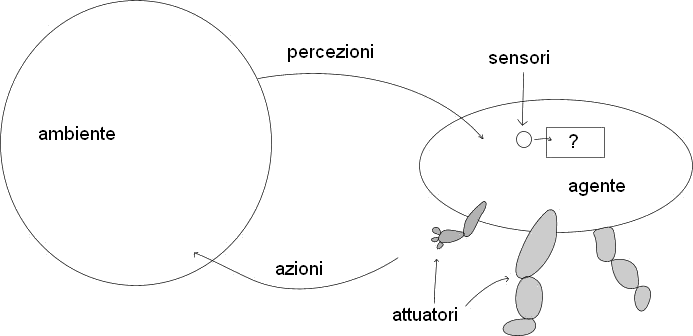
\includegraphics[width=\textwidth,height=\textheight,keepaspectratio]{Figures/Vario/Agente.png}
\caption[Interazione di un agente con l'ambiente esterno]{Interazione di un agente con l'ambiente esterno}
\label{fig:Agente}
\end{figure}

\noindent Nel campo dell'Intelligenza artificiale un obiettivo fondamentale è la realizzazione degli agenti intelligenti (o agenti razionali). Nella fattispecie un agente si definisce intelligente se fa la cosa giusta al momento giusto.\\

\noindent Per poter stabilire questo occorre fornire una qualche misura delle prestazioni. In particolare è importante definire il come e il quando eseguire la valutazione delle azioni. Perciò si rende necessario un modello di successo, stabilito a priori, con il quale confrontare i risultati ottenuti. \cite{AgenteIntelligente}

\newpage
	
\noindent È possibile raggruppare gli agenti in 5 classi in base al grado di intelligenza percepita e alle capacità: \cite{AgenteIntelligente} \label{Agente}
\begin{itemize}
\item agenti con riflessi semplici (detti anche puramente reattivi);
\item agenti con riflessi basati su modello;
\item agenti basati su obiettivo;
\item agenti basati su utilità;
\item agenti che apprendono;
\end{itemize}

\noindent Per questo lavoro andremo a considerare la prima categoria riportata nell'elenco, ovvero agenti con riflessi semplici. Questa funzione d'agente infatti si comporta bene nel caso in cui l'ambiente sia completamente osservabile, come appunto sarà possibile fare in questo caso.

\subsection{Sistema}
Prima di comprendere il termine "sistema complesso" bisogna andare a capire cos'è un sistema. Esistono varie definizioni di questo termine, che dipendono principalmente dal contesto in cui viene utilizzato. Generalmente però si può definire un sistema come un gruppo di oggetti interagenti oppure indipendenti che fanno parte di un tutt'uno. Notare che i limiti di un sistema non sono sempre ben definiti.\\
Si può catalogare un sistema in base anche alla sua complessità strutturale ed operazionale, come ad esempio nelle seguenti tre categorie:
\begin{itemize}
\item Sistema semplice: conosciuto e basato su causa-effetto (bicicletta)
\item Sistema complicato: richiede conoscenza ma è studiabile (macchina)
\item Sistema complesso: non conosciuta e che richiede ricerca, simulazione e analisi (comportamento di un organismo)
\end{itemize}

\newpage

\subsection{Sistema complesso}
Innumerevoli definizioni possono essere associate al termine "sistema complesso"; in generale si può dire che un sistema complesso è un sistema strutturato, difficile sia da comprendere sia da testare, in cui ci sono diverse interazioni tra le componenti al suo interno. Inoltre, un sistema complesso è molto sensibile ad eventuali variazioni della situazione iniziale. Uno degli scopi principali per cui si realizzano questi sistemi è la simulazione, e alcuni esempi di sistemi complessi sono: \cite{SistemaComplesso}
\begin{itemize}
\setlength\itemsep{0.1em}
\item Automi cellulari
\item Crosta terrestre e interazioni che provocano i terremoti
\item Sistema climatico
\item Sistemi sociali
\item Sistemi economici
\item Ambiente e territorio
\end{itemize}

\subsection{Simulazione sistema}
Rappresenta un modo di sfruttare modelli computazionali con lo scopo di valutare la scelta di piani, design, teorie e/o modelli. Spesso è necessario ricorrere ad un ambiente sintetico perchè il sistema reale può non essere facilmente osservabile.

\begin{figure}[ht]
\centering
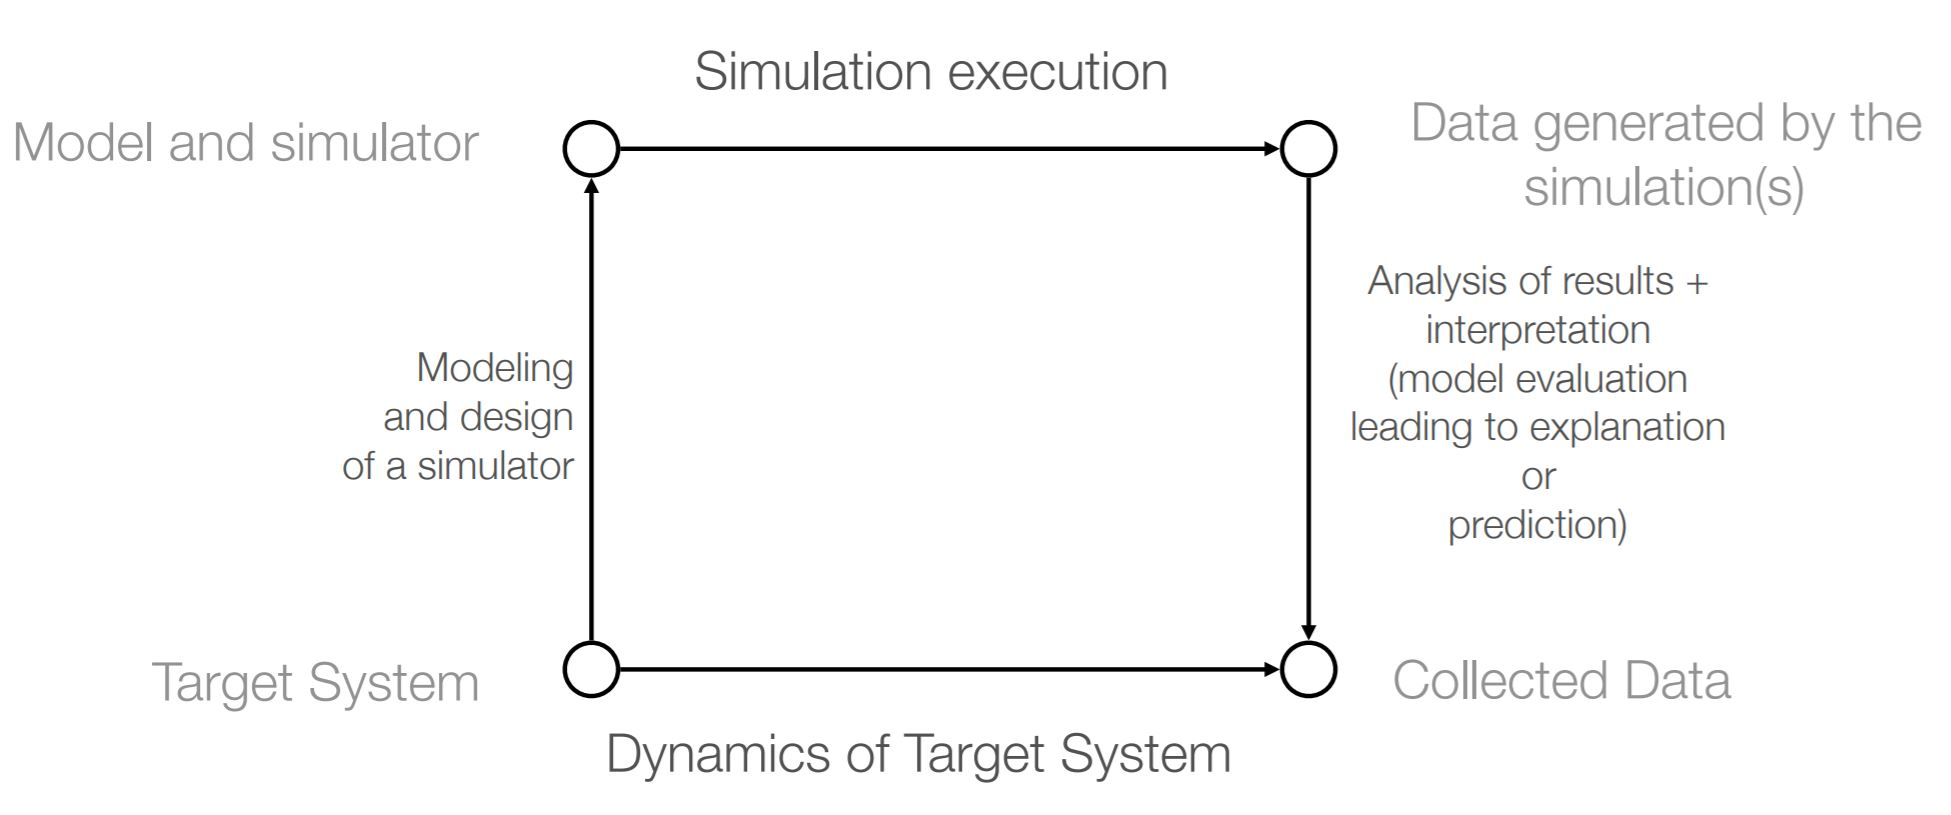
\includegraphics[width=0.9\textwidth,height=\textheight,keepaspectratio]{Figures/Vario/Simulazione.jpg}
\caption[Ciclo di vita di una simulazione]{Ciclo di vita di una simulazione}
\label{fig:Simulazione}
\end{figure}

\newpage

\subsection{Sistema multiagente}
Un sistema multiagente o (sistema ad agenti multipli) è un insieme di agenti situati in un certo ambiente ed interagenti tra loro mediante una opportuna organizzazione. Un agente è cioè un'entità caratterizzata dal fatto di essere, almeno parzialmente, autonoma, sia essa un programma informatico, un robot, un essere umano, e così via.

\begin{figure}[ht]
\centering
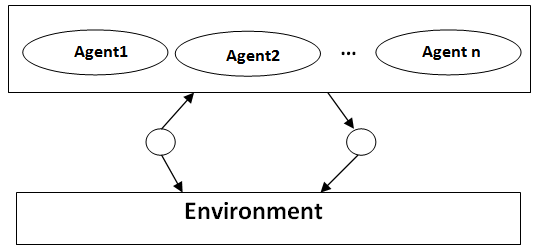
\includegraphics[width=0.9\textwidth,height=\textheight,keepaspectratio]{Figures/Vario/MAS.png}
\caption[Interazione di più agenti con l'ambiente]{Interazione di più agenti con l'ambiente}
\label{fig:MAS}
\end{figure}

\noindent Oggetto di ricerche da lunga data in intelligenza artificiale, i sistemi ad agenti multipli costituiscono un'interessante tipologia di modellazione di società, e hanno a questo riguardo vasti campi d'applicazione, che si estendono fino alle scienze umane e sociali (economia, sociologia, etc.). \cite{SistemaMultiagente}\\

\noindent Un sistema multiagente, per essere definito tale, deve rispettare le seguenti caratteristiche: \cite{CaratteristicheMAS}
\begin{itemize}
\item Autonomia: ogni agente deve essere almeno parzialmente indipendente.
\item Vista locale: nessun agente deve avere la vista globale del sistema.
\item Decentralizzazione: nessun agente può controllare l'intero sistema.
\end{itemize}

\newpage
\subsubsection{Modelli di interazione tra agenti}
Due o più agenti interagiscono tra loro se sono in una relazione dinamica attraverso sequenza di azioni reciproche. Due agenti sono portati ad interagire tra di loro quando non è possibile effettuare o portare a termine un determinato compito da parte di un agente singolo. Ciò può accadere a causa di risorse insufficienti, abilità insufficienti oppure per un approccio distribuito.\\

\noindent Esistono diversi modelli di interazione tra agenti, che possono essere suddivisi a loro volta in due grandi categorie: modelli di interazione diretta e modelli di interazione indiretta.

\begin{figure}[ht]
\centering
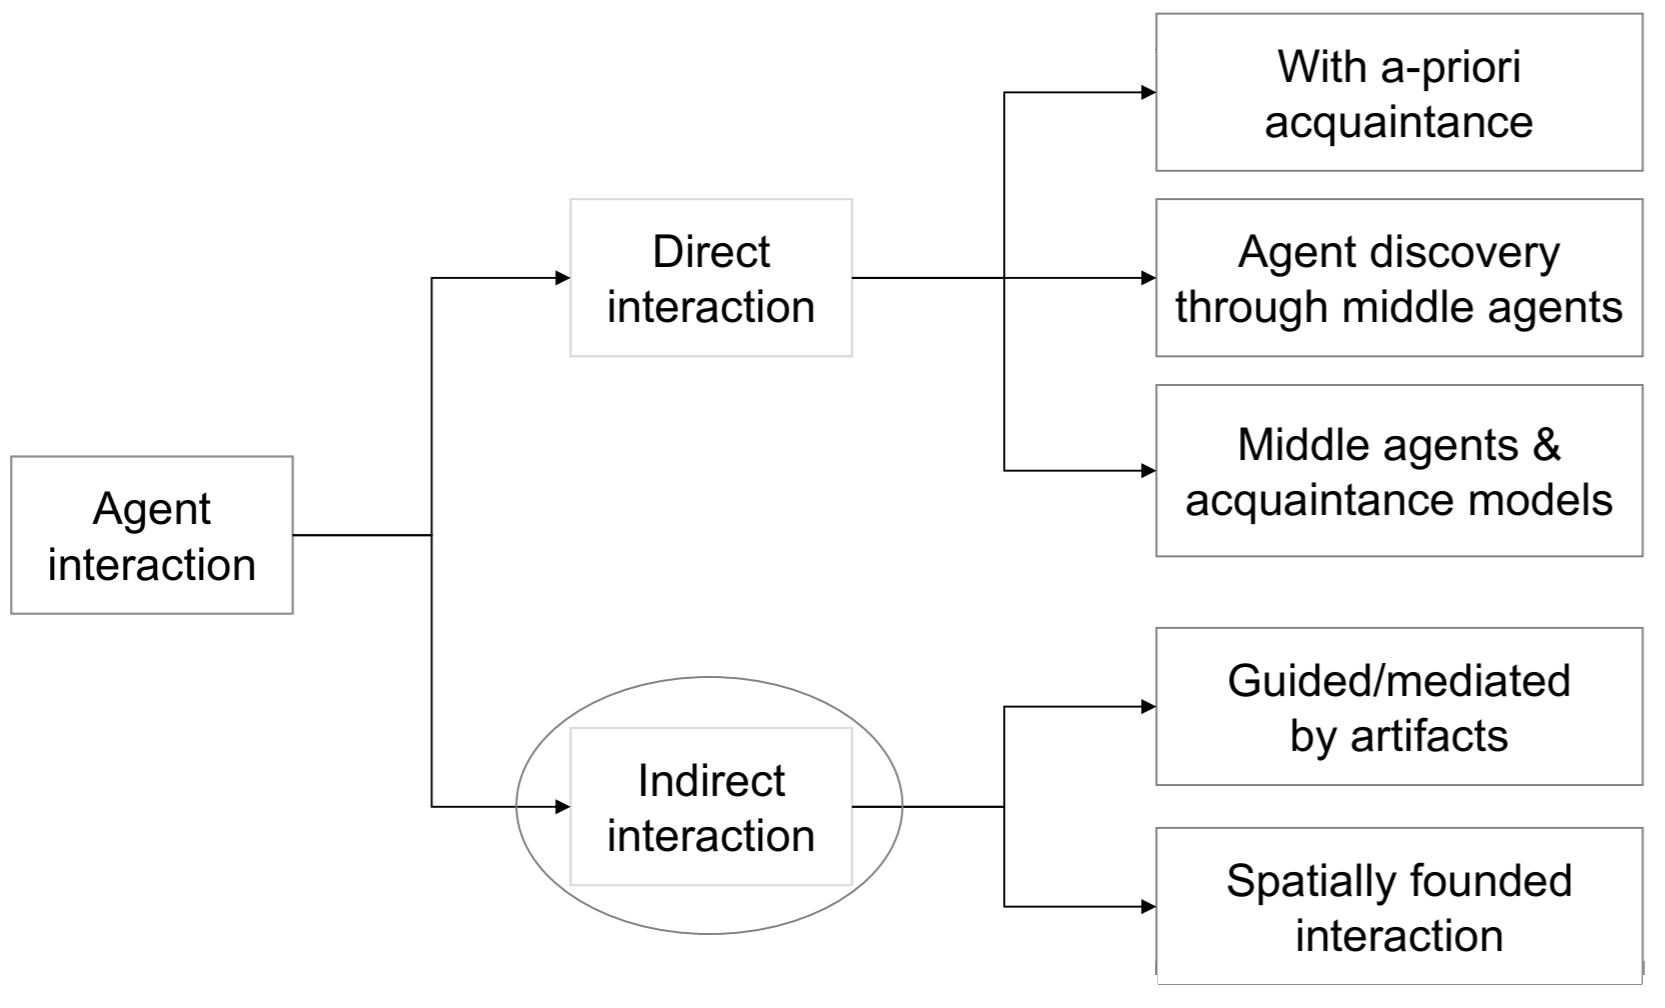
\includegraphics[width=\textwidth,height=\textheight,keepaspectratio]{Figures/Vario/Agent_Interaction.png}
\caption[Modelli di interazione tra agenti]{Modelli di interazione tra agenti}
\label{fig:Agent_Interaction}
\end{figure}

\noindent Nei modelli ad interazione diretta gli agenti sono in grado di comunicare direttamente tra di loro. Lo scambio di informazioni è reso possibile grazie all'utilizzo di un agent communication language (ACL) e di una struttura dei messaggi. La comunicazione tra due agenti di questo genere avviene quindi maniera indiscriminata dato che l'informazione va dal mittente al destinatario senza alcun tipo di dispersione e/o intermediario esterno. \\ Questi modelli sono facilmente implementabili e simili a sistemi distribuiti già esistenti, anche se allo stesso tempo sono presenti regole strette sul metodo di comunicazione e ogni agente deve essere a conoscenza di un altro agente prima di poterci comunicare.\\

\noindent Nei modelli ad interazione indiretta invece gli agenti interagiscono attraverso un ente che funziona di intermediario. Questo ente fornisce dei meccanismi di comunicazioni e delle regole dia accesso. L'implementazione di un modello del genere permette di avere un'interazione mediata, e quindi maggior possibilità di controllo, seppur l'implementazione risulta molto complessa per alcuni contesti e alcuni sistemi distribuiti.


\subsubsection{Tipologie di ambienti}
\noindent Un sistema multiagente consiste negli agente e del relativo ambiente. Le diverse categorie di agenti sono già state riportate nella sezione precedente \ref{Agente}, mentre per quanto riguarda l'ambiente può essere suddiviso in:


\begin{table}[ht]
\centering
\resizebox{\textwidth}{!}{%
\begin{tabular}{lll}
\multicolumn{1}{c}{\cellcolor[HTML]{EFEFEF}\textbf{Accessible}}                                                                                                                                             &  & \multicolumn{1}{c}{\cellcolor[HTML]{EFEFEF}\textbf{Inaccessible}}                                                                                                                      \\
\begin{tabular}[c]{@{}l@{}}E' possibile conoscere tutte le informazioni \\ riguardanti le possibili combinazione \\ dell'evoluzione dell'ambiente.\end{tabular}                                             &  & \begin{tabular}[c]{@{}l@{}}Non è possibile conoscere tutte le informazioni \\ riguardanti le possibili combinazione \\ dell'evoluzione dell'ambiente.\end{tabular}                     \\
                                                                                                                                                                                                            &  &                                                                                                                                                                                        \\
\multicolumn{1}{c}{\cellcolor[HTML]{EFEFEF}\textbf{Deterministic}}                                                                                                                                          &  & \multicolumn{1}{c}{\cellcolor[HTML]{EFEFEF}\textbf{Non Deterministic}}                                                                                                                 \\
\begin{tabular}[c]{@{}l@{}}E' possibile conosce in maniera deterministica \\ tutti i cambiamenti che una certa azione \\ porta al sistema.\end{tabular}                                                     &  & \begin{tabular}[c]{@{}l@{}}Non è possibile conosce in maniera \\ deterministica tutti i cambiamenti che \\ una certa azione porta al  sistema.\end{tabular}                            \\
                                                                                                                                                                                                            &  &                                                                                                                                                                                        \\
\multicolumn{1}{c}{\cellcolor[HTML]{EFEFEF}\textbf{Episodic}}                                                                                                                                               &  & \multicolumn{1}{c}{\cellcolor[HTML]{EFEFEF}\textbf{Non Episodic}}                                                                                                                      \\
\begin{tabular}[c]{@{}l@{}}Le performance di un agente dipendono dal \\ numero di episodi discreti avvenuti,  con nessun\\ rapporto con le performance dell'agente \\ in uno scenario diverso.\end{tabular} &  & \begin{tabular}[c]{@{}l@{}}Le performance di un agente non dipendono \\ dal numero di episodi discreti avvenuti, \\ e l'agente prende decisioni su \\ scenari differenti.\end{tabular} \\
                                                                                                                                                                                                            &  &                                                                                                                                                                                        \\
\multicolumn{1}{c}{\cellcolor[HTML]{EFEFEF}\textbf{Static}}                                                                                                                                                 &  & \multicolumn{1}{c}{\cellcolor[HTML]{EFEFEF}\textbf{Dynamic}}                                                                                                                           \\
\begin{tabular}[c]{@{}l@{}}Non è soggetto a variazioni sul suo stato \\ durante il corso della finestra temporale\\ in cui l'agente sta agendo.\end{tabular}                                                &  & \begin{tabular}[c]{@{}l@{}}E' soggetto a variazioni sul suo stato \\ durante il corso della finestra temporale \\ in cui l'agente sta agendo.\end{tabular}                             \\
                                                                                                                                                                                                            &  &                                                                                                                                                                                        \\
\multicolumn{1}{c}{\cellcolor[HTML]{EFEFEF}\textbf{Discrete}}                                                                                                                                               &  & \multicolumn{1}{c}{\cellcolor[HTML]{EFEFEF}\textbf{Continuous}}                                                                                                                        \\
\begin{tabular}[c]{@{}l@{}}E' possibile rappresentare con una \\ cardinalità finita gli stati dell'ambiente.\end{tabular}                                                                                   &  & \begin{tabular}[c]{@{}l@{}}Non è possibile rappresentare con una \\ cardinalità finita gli stati dell'ambiente.\end{tabular}                                                          
\end{tabular}%
}
\caption{Diverse tipologie di ambiente}
\label{Ambiente}
\end{table}

\newpage

\subsection{Automated Guided Vehicle}
Un veicolo a guida autonoma (AGV) identifica dei veicoli, solitamente utilizzati in campo industriale per il trasporto di prodotti da un punto dello stabilimento ad un altro.\\

\begin{figure}[ht]
\centering
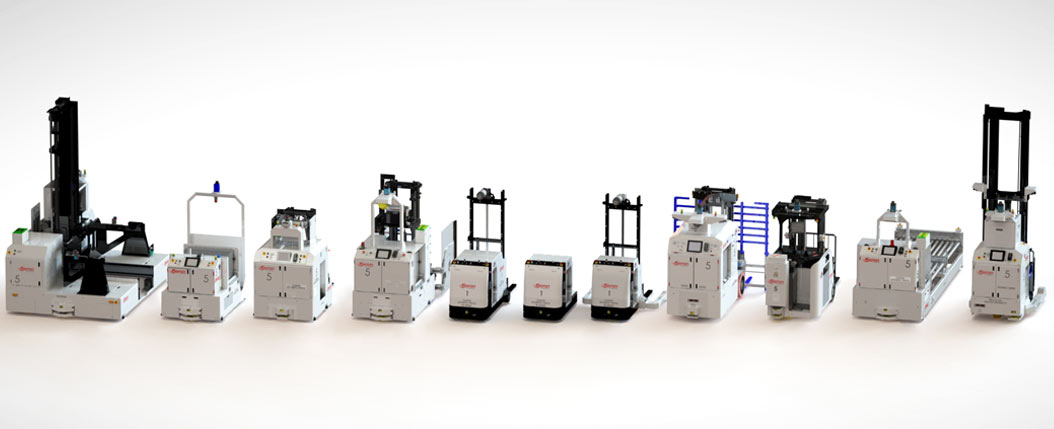
\includegraphics[width=\textwidth,height=\textheight,keepaspectratio]{Figures/Vario/AGV.jpg}
\caption[Diversi modelli di AGV]{Diversi modelli di AGV}
\label{fig:AGV}
\end{figure}


\noindent Esistono numerose tecnologie adottate per la realizzazione di AGV, ognuna con vantaggi e svantaggi; la scelta tecnica di realizzazione infatti è fortemente correlata al problema e all'ambiente che si sta considerando.  degli AGV:
\begin{table}[ht]
\centering
\resizebox{0.8\textwidth}{!}{%
\begin{tabular}{lll}
\multicolumn{1}{c}{\cellcolor[HTML]{EFEFEF}\textbf{Navigation}}                                                                                                                         &                               & \multicolumn{1}{c}{\cellcolor[HTML]{EFEFEF}\textbf{Path decision}}                                                        \\
\begin{tabular}[c]{@{}l@{}}- Wired\\ - Guide tape\\ - Laser target navigation\\ - Inertial navigation\\ - Natural features navigation \\ - Vision guidance\\ - Geoguidance\end{tabular} &                               & \begin{tabular}[c]{@{}l@{}}- Frequence select mode\\ - Path select mode\\ - Magnetic tape mode\end{tabular}               \\
                                                                                                                                                                                        &                               &                                                                                                                           \\
\multicolumn{1}{c}{\cellcolor[HTML]{EFEFEF}\textbf{Traffic control}}                                                                                                                    & \multicolumn{1}{c}{\textbf{}} & \multicolumn{1}{c}{\cellcolor[HTML]{EFEFEF}\textbf{Battery charging}}                                                     \\
\begin{tabular}[c]{@{}l@{}}- Zone control\\ - Collision avoidance\\ - Combination control\end{tabular}                                                                                  &                               & \begin{tabular}[c]{@{}l@{}}- Battery swap\\ - Automatic and opportunity charging \\ - Automatic battery swap\end{tabular}
\end{tabular}%
}
\caption{Diverse tipologie di tecnologie utilizzate per realizzazione AGV}
\label{AGVchars}
\end{table}


\newpage

\subsection{Automated Guided Vehicle System}
\noindent Un sistema automatizzato di veicoli a guida autonoma (AGVS) permette una gestione estremamente flessibile per spedizione e gestione di materiali, soprattutto per quegli ambienti in cui i prodotti sono molto vari e le necessità continuano a variare nel tempo. \\

\noindentQuesti sistemi sono stati introdotti nel 1950, e da allora si sono trovati sempre più contesti e applicazioni in cui forniscono un'elevata utilità pratica. Inoltre, con l'avvento di tecnologie sempre più avanzate e di MAS sempre più sofisticati, le performance di questi sistemi sono in continua crescita.

\subsubsection{Classificazione di un AGVS}
Un AGVS deve essere progettato e implementato considerando il contesto in cui ci si trova e le priorità che si presentano. Tutto sommato, un AGVS può essere classificato in base ai tre seguenti requisiti:
\begin{itemize}
\item \textbf{Percorso di guida:} Può essere statico, in cui la navigazione avviene seguendo una serie di percorsi prestabiliti (unidirezionale o bidirezionale) oppure può essere dinamico, in cui la navigazione dei veicoli avviene in maniera completamente autonoma.

\item \textbf{Capacità del veicolo:} Un AGV può avere una capacità di carico diversa da un altro, come ad esempio carico unitario e carico multiplo.

\item \textbf{Indirizzamento dei veicoli:} L'indirizzamento dei veicoli può essere indiretto, in cui un AGV può visitare solamente determinate stazioni, oppure diretto, in cui ogni AGV può visitare ogni stazione.

\end{itemize}

\subsubsection{Performance di un AGVS}
Solitamente la valutazione delle performance di un AGVS avviene tramite simulazione che, attraverso la raccolta di parametri rilevanti, permette di misurare le performance di un sistema rispetto ad un altro. Esempi di parametri di produzione che possono essere valutati di un AGVS sono:
\begin{itemize}
\setlength\itemsep{0.1em}
    \item Ordini svolti
    \item Tempo medio di attesa per ordini pronti
    \item Coda di ordini in attesa
    \item Numero di conflitti
    \item Numero di deadlock
    \item Numero totale di AGV impiegati
    \item Tempo totale di utilizzo degli AGV
    \item Tempo in cui un AGV è impiegato di un azione
    \item Tempo in cui un AGV non è impiegato in nessuna azione
\end{itemize}

\subsection{Lavori precedenti}
Nonostante svariati lavori sono stati già ampliamenti portati a termine e documentati non è risultato del tutto facile ed intuitivo trovare dei lavori su cui basare le nostre scelte implementative e progettuali.\\

\noindent Nonostante ciò alcuni lavori ci sono tornati estremamente utili per delle sottosezioni del progetto; ad esempio il lavoro documentato all'interno dell'articolo scientifico "Evaluation of automatic guided vehicle systems" \cite{EvaluationAGVS} ci ha permesso di individuare e definire le metriche utili alla valutazione del nostro simulatore. \noindent Un altro articolo scientifico di estrema utilità è risultato essere "Multi Agent Simulation for Decision Making in Warehouse Management"\cite{MAS_Warehouse}, in cui viene analizzato e simulato un sistema su un ambiente molto simile a quello affrontato da questo studio.

\newpage
%%%%%%%%%%%%%%%%%%%%%%%%%%%%%%%%%%%%%%%%%%%%%%%
% Descrizione del dominio
%%%%%%%%%%%%%%%%%%%%%%%%%%%%%%%%%%%%%%%%%%%%%%%
\section{Descrizione del dominio}
\subsection{Azienda}
LDE s.r.l nasce nel 1997 come azienda per il trasporto e la logistica specializzata in abiti e tessuti. Ad oggi conta circa 30 dipendenti e un fatturato di oltre un milione di euro. Si è entrati in contatto con questa azienda grazie ad una collaborazione passata.

\subsection{Tipologia di lavoro e di ordini}
Il lavoro svolto da questa azienda consiste principalmente nell'elaborazione, preparazione, ricezione e spedizione di articoli. Gli articoli in questione possono essere di svariati tipi, dai vestiti agli accessori, da macchinari a utensili da cucina,..
In questo studio si andrà a considerare la parte del magazzino che tratta gli ordini inerenti agli articoli in ambito vestiario da loro trattati.

\subsection{Ambiente}
L'ambiente del magazzino preso da noi in considerazione consta di una zona per gli uffici (in basso a sinistra), 4 gate per caricare i camion (di cui uno chiuso, motivo per cui ne sono stati rappresentati tre sulla mappa della simulazione) e 8 corsie in cui sono posizionate le merci. Nella simulazione, tutto è rappresentato in scala 1:1 con piccole approssimazioni che non influiscono né sulle performance, né sull'aderenza alla realtà della simulazione.
Per quanto riguarda l'ambiente, le uniche assunzione che sono state fatte riguardano gli oggetti e, in particolare:
\begin{itemize}
    \item Gli oggetti nel magazzino sono sempre disponibili per un AGV che li richiede.
    \item Un AGV prende un oggetto posizionandosi in un punto preciso per la ricezione di quell’oggetto che viene posizionato sull’AGV da un ipotetico braccio meccanico.
\end{itemize}

\noindent Di seguito è riportata la cartina rappresentante la perimetria del dominio in questione, che verrà utilizzata nella fasi successive per ottenere un ambiente di simulazione verosimile a quello reale.

\begin{figure}
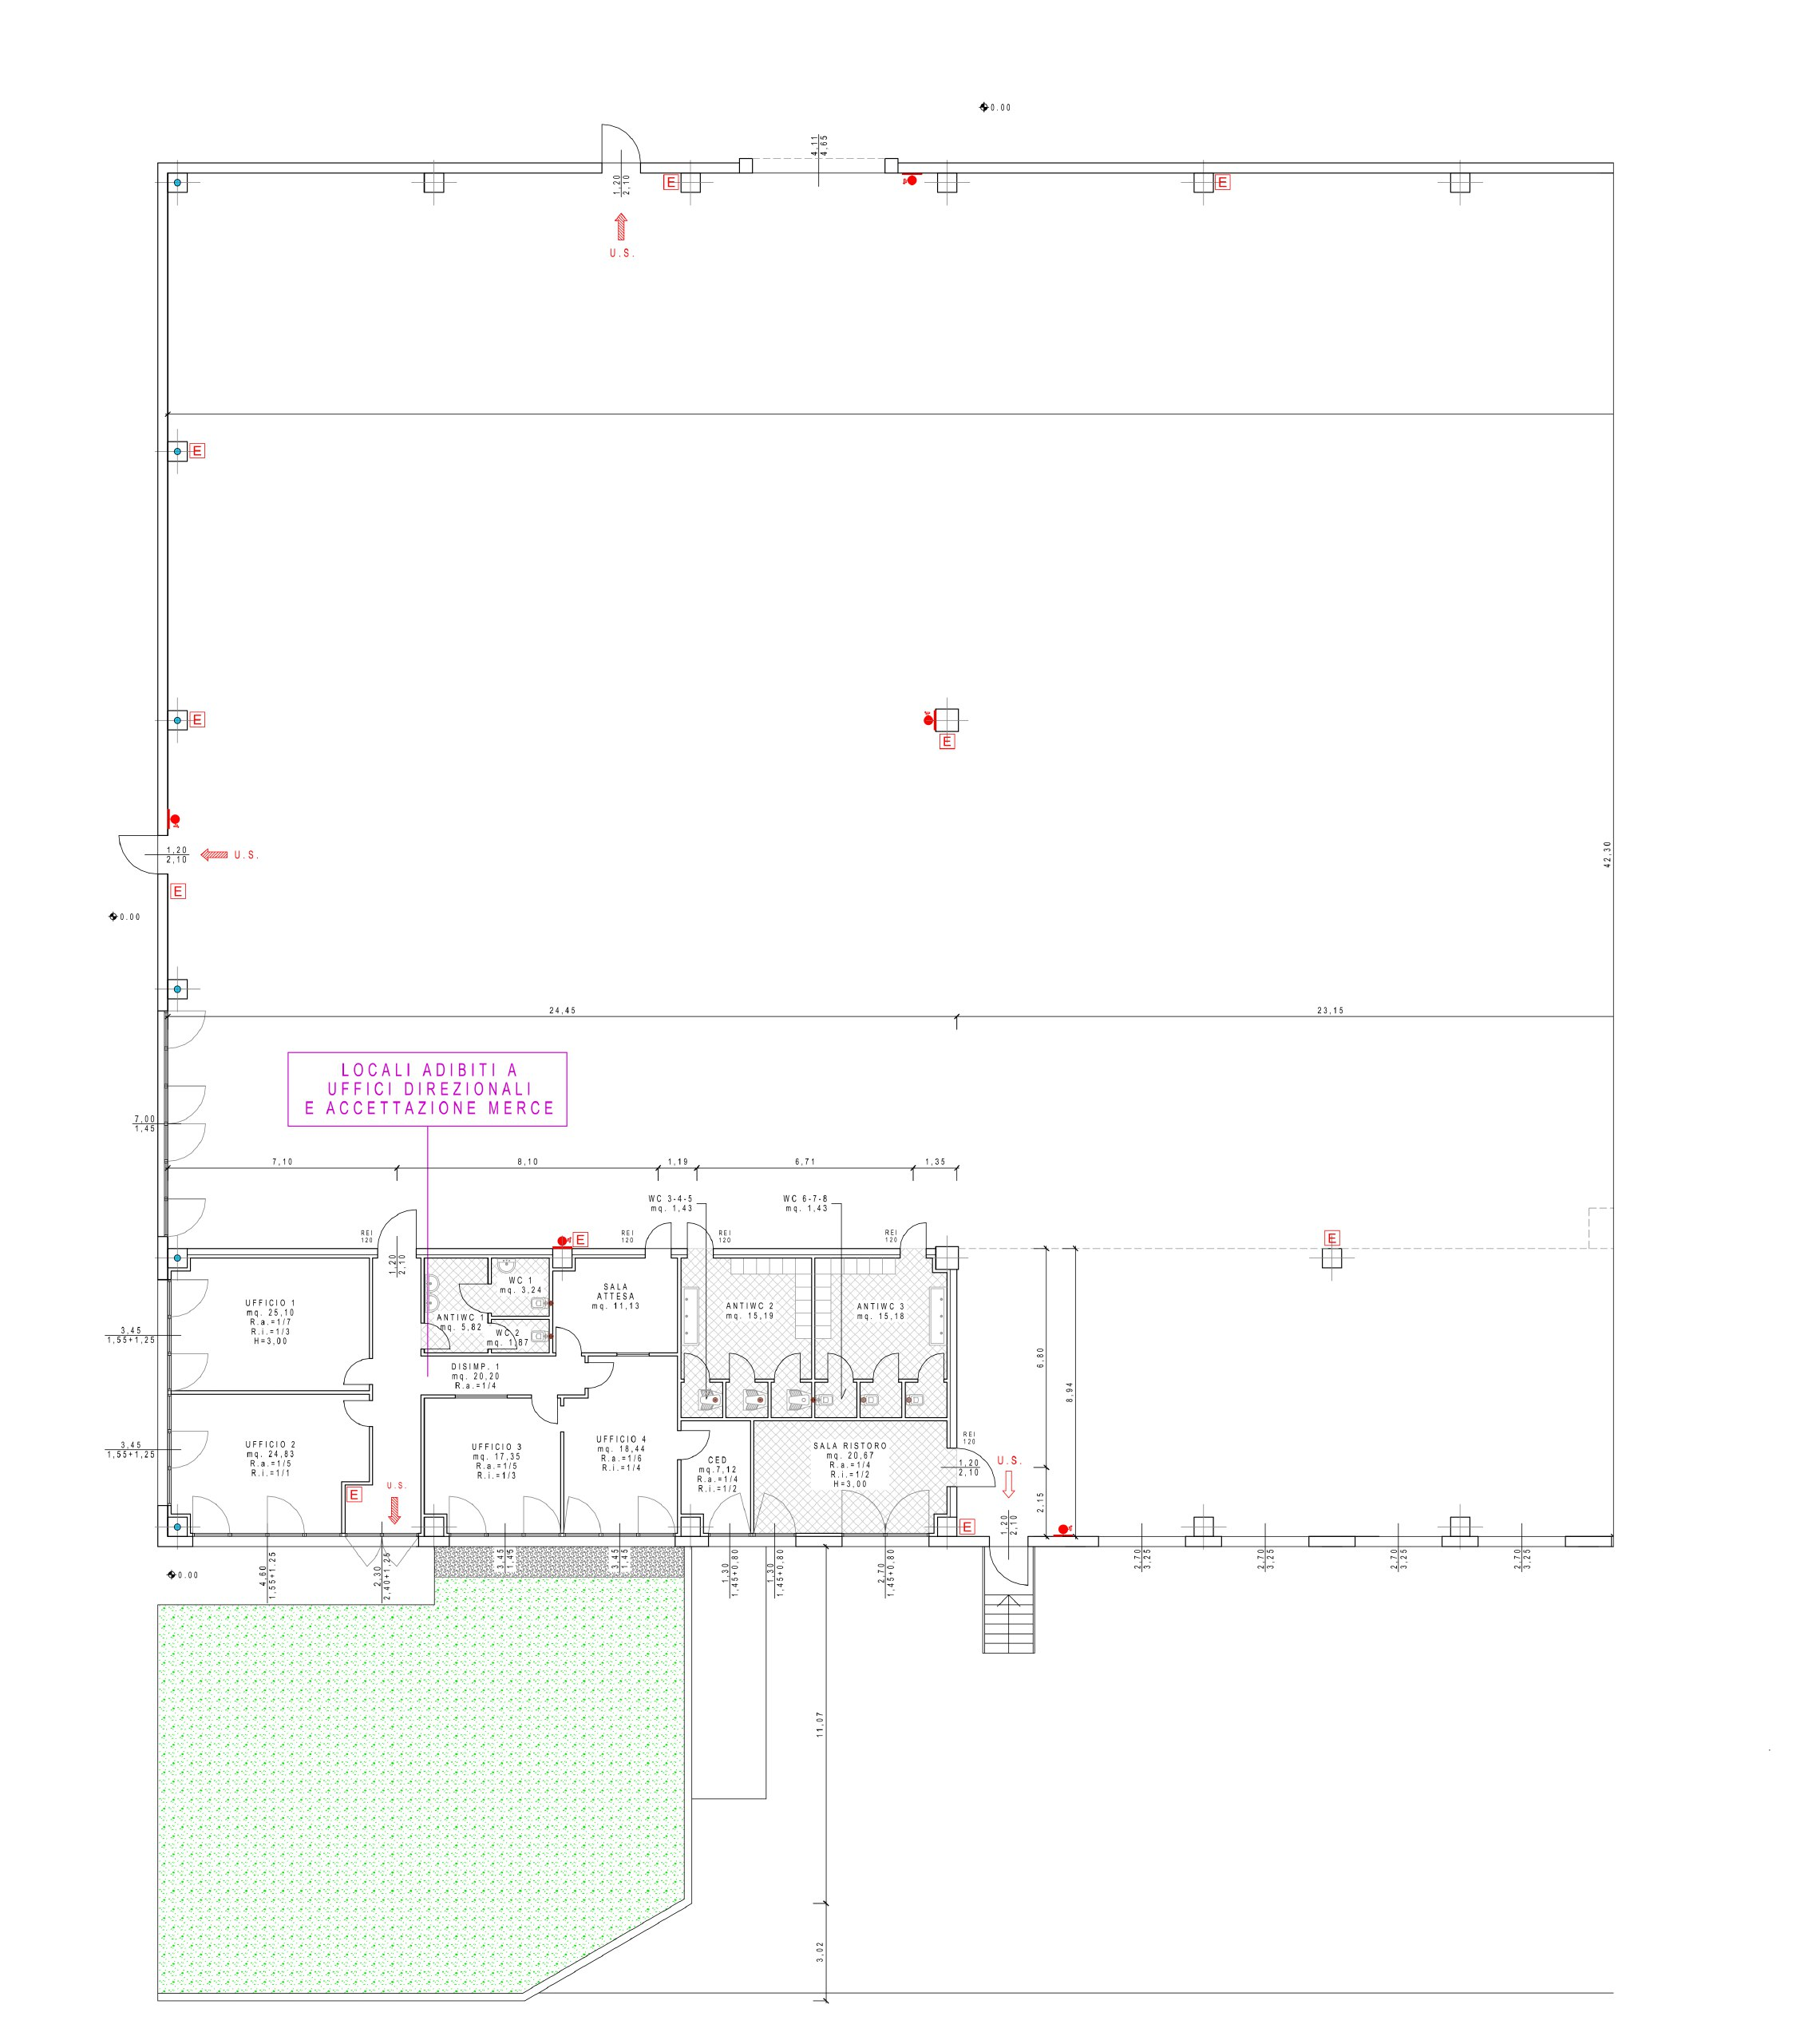
\includegraphics[width=\textwidth,height=\textheight,keepaspectratio]{Figures/Graphics/Zoom_Map.jpg}
\caption[Mappa fisica del magazzino]{Mappa fisica del magazzino}
\label{fig:Mappa_magazzino}
\end{figure}


\subsection{Lista degli ordini}
Insieme alla cartina del magazzino è stato possibile reperire un elenco di ordini che vengono svolti quotidianamente; la lista di cui si sta parlando contiene 2023 ordini differenti. Ciascun ordine contiene una lista di articoli che può variare e un unico destinatario, che può essere:
\begin{itemize}
\item Milano (MI)
\item Firenze (FI)
\item Como (CO)
\end{itemize}
Il seguente grafico riporta il numero di ordini presenti all'interno della lista per ciascuna destinazione.

\begin{figure}[ht]
\centering
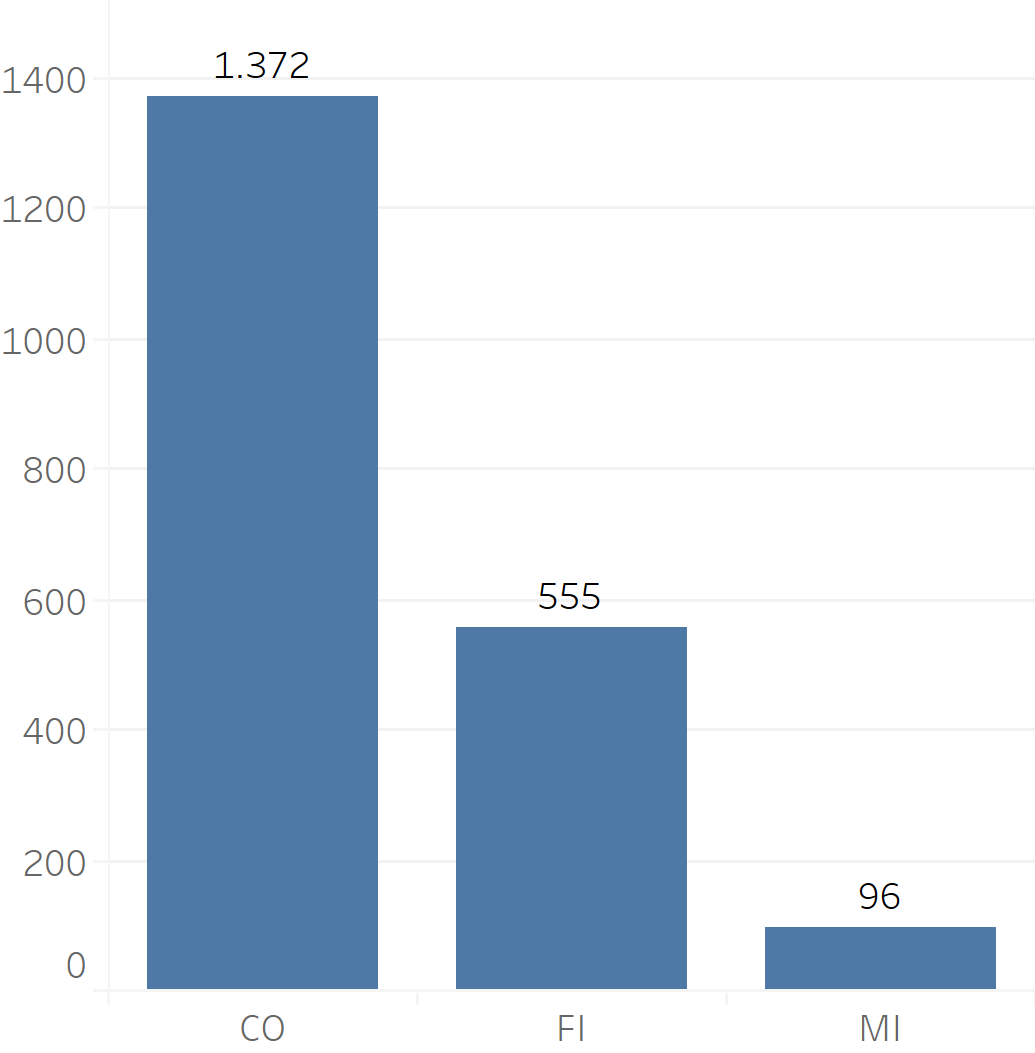
\includegraphics[width=0.7\textwidth,height=\textheight,keepaspectratio]{Figures/Initial_Dataset/Orders_client.png}
\caption[Numero di ordini per ciascun cliente]{Numero di ordini per ciascun cliente}
\label{fig:OrdiniClientiIniziali}
\end{figure}


\newpage
%%%%%%%%%%%%%%%%%%%%%%%%%%%%%%%%%%%%%%%%%%%%%%%
% Modellazione del problema
%%%%%%%%%%%%%%%%%%%%%%%%%%%%%%%%%%%%%%%%%%%%%%%
\section{Modellazione del problema}

\subsection{Ambiente del simulatore}
Una volta ottenuta la mappa del magazzino, si è andati a cercare di rappresentare la struttura del magazzino in maniera tale da renderla utilizzabile per un sistema di simulazione.
\begin{figure}[ht]
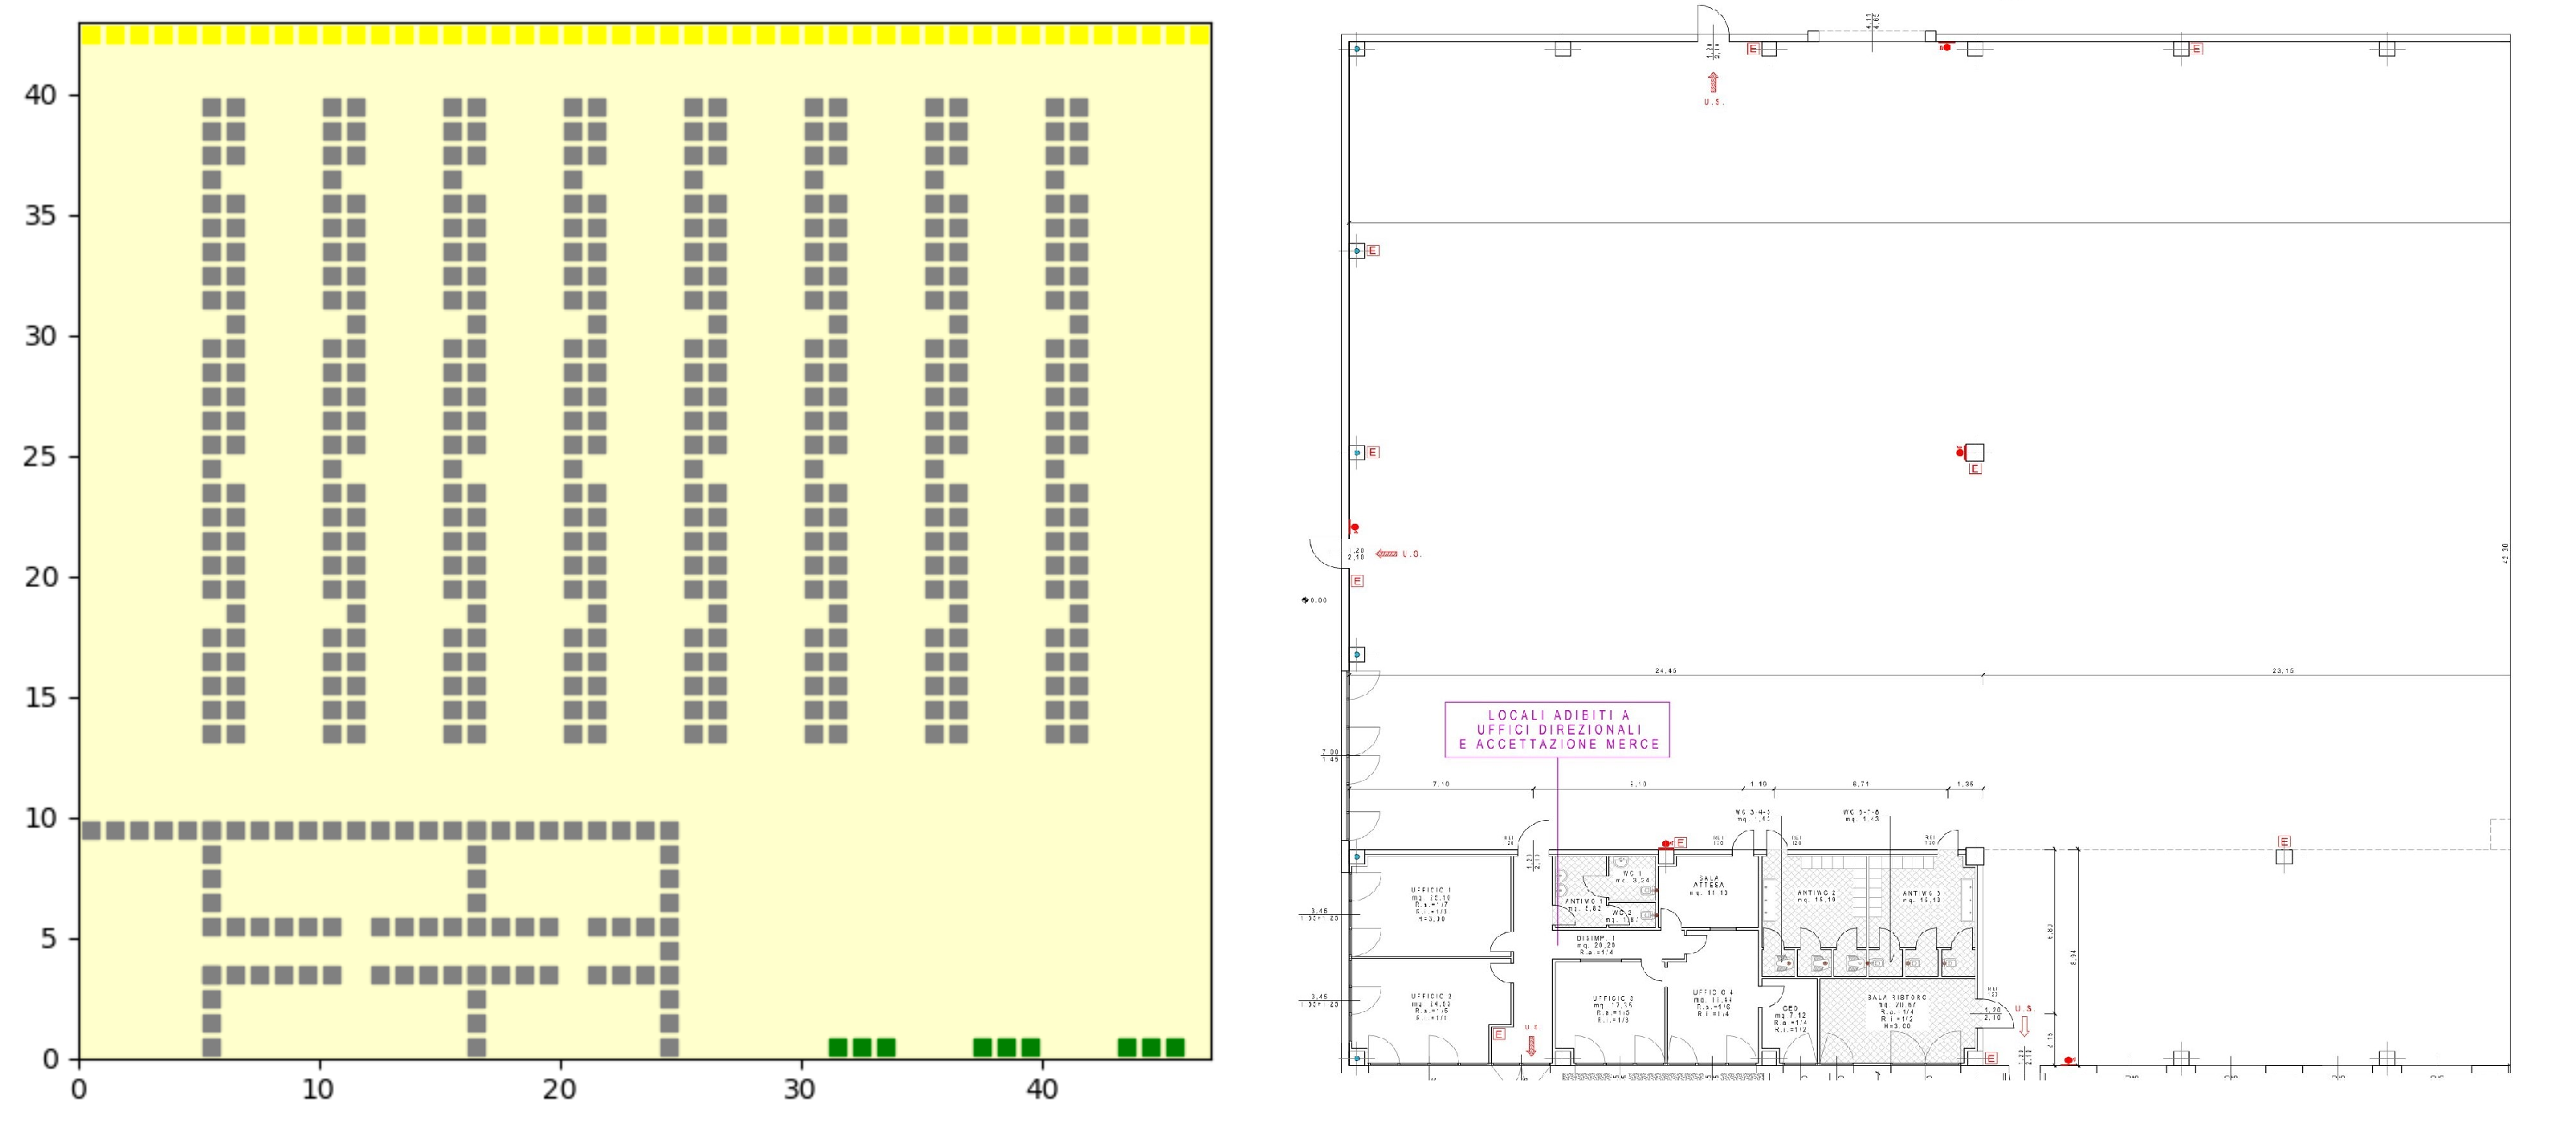
\includegraphics[width=\linewidth]{Figures/Graphics/Simulation_Domain.PNG}
\caption{Rappresentazione della mappa del magazzino sul simulatore}\label{fig:Rappresentazione_mappa}
\end{figure}

\noindent All'interno dell'ambiente sono stati definiti i seguenti elementi, di cui i primi 4 sono quelli fondamentali alla simulazione del problema e meglio descritti nella pagina seguente:

\begin{itemize}
\item Scaffalature
\item Punti di carico
\item Punti di scarico
\item Area di attesa
\item Area di ricarica
\item Uffici:
\end{itemize}
\newpage


\begin{minipage}[ht]{0.45\linewidth}
\centering
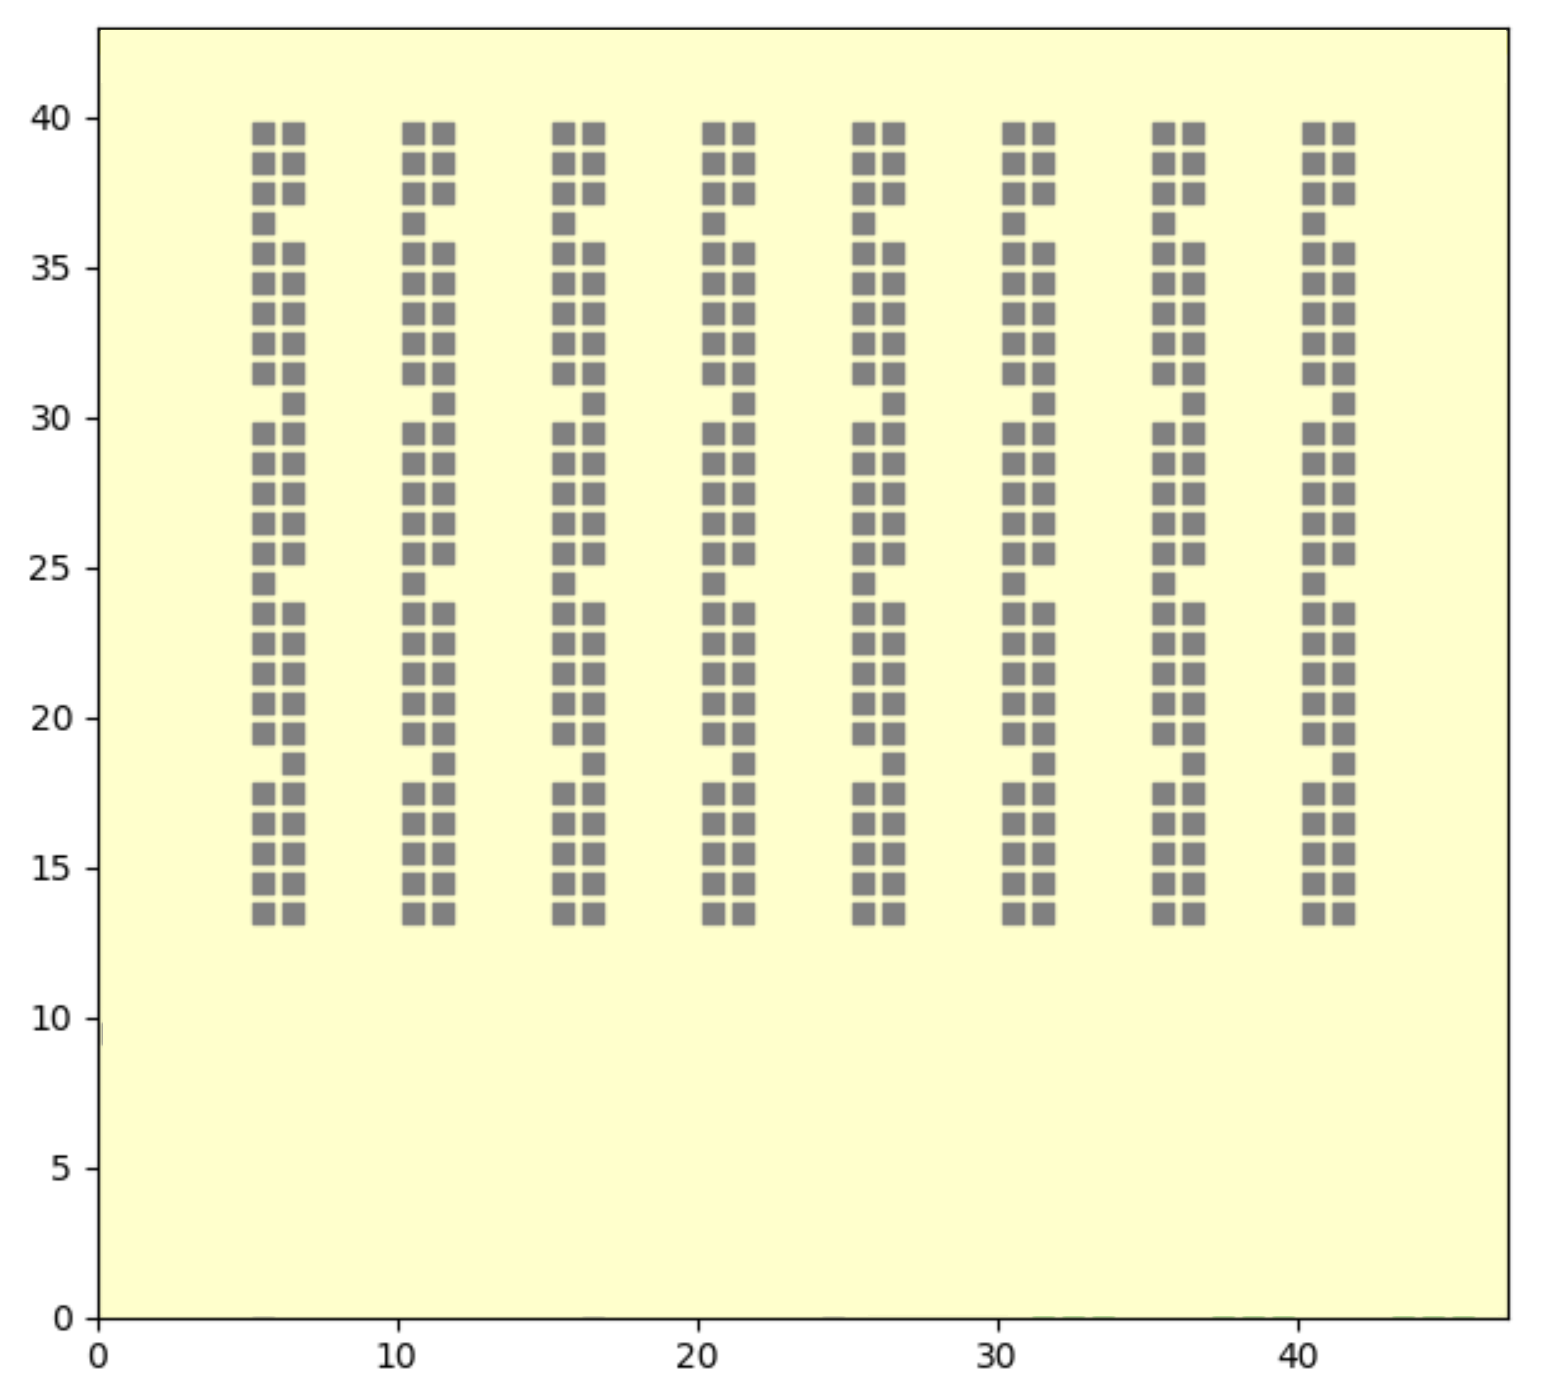
\includegraphics[width=\textwidth]{Figures/Map/Corsie.png}
\end{minipage}
\hspace{0.5cm}
\begin{minipage}[ht]{0.45\linewidth}
\centering
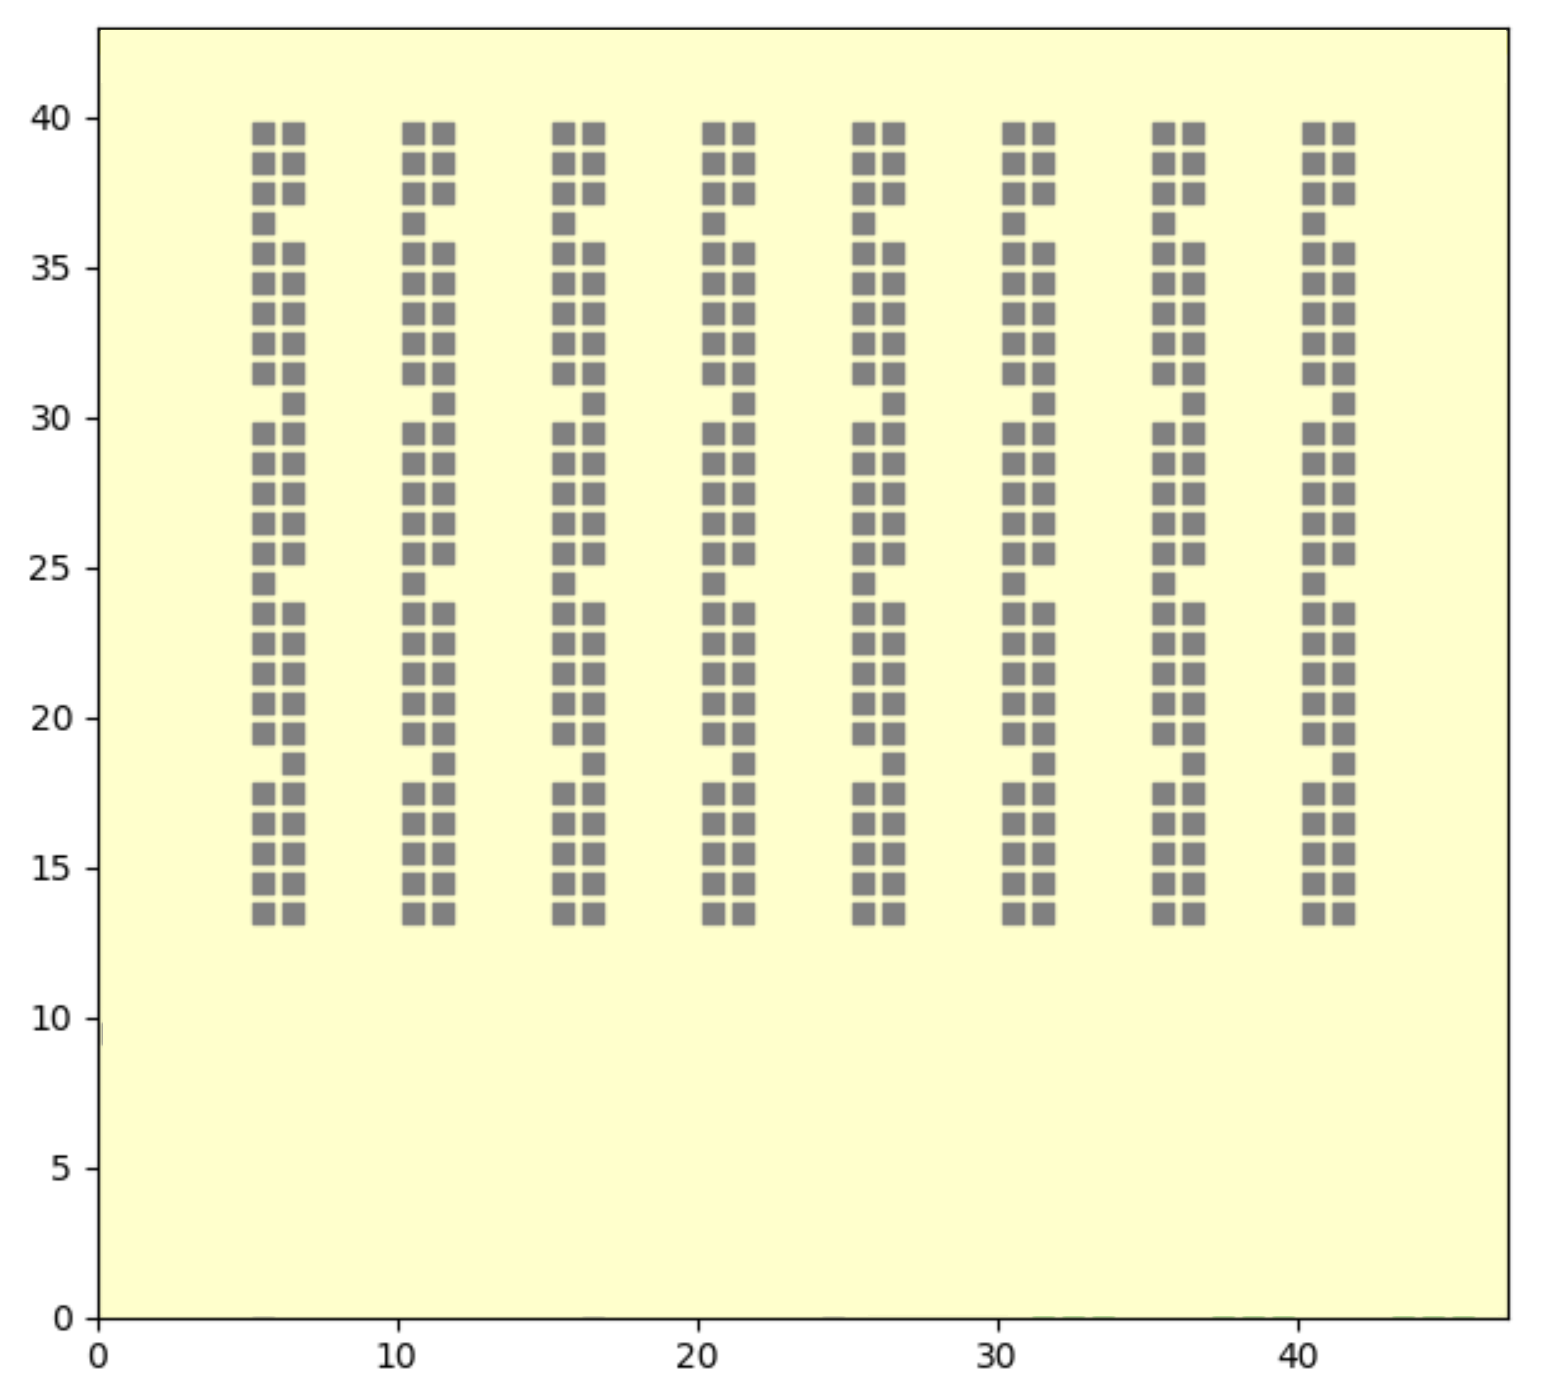
\includegraphics[width=\textwidth]{Figures/Map/Corsie.png}
\end{minipage}

\begin{minipage}[ht]{0.45\linewidth}
\vspace{0.2cm}
\textbf{Scaffalature:} Rappresentate con il colore grigio al centro dell'ambiente di simulazione, rispecchiando le corrispettive 8 scaffalature presenti all'interno del magazzino fisico.
\end{minipage}
\hspace{0.5cm}
\begin{minipage}[ht]{0.45\linewidth}
\vspace{0.2cm}
\textbf{Punti di carico:} Rappresentati con delle interruzioni della corsia sono collocati lungo le corsie stesse, dove l'AGV potrà accedere per poter prelevare le merci richieste.
\end{minipage}

\vspace{1cm}
\begin{minipage}[ht]{0.45\linewidth}
\centering
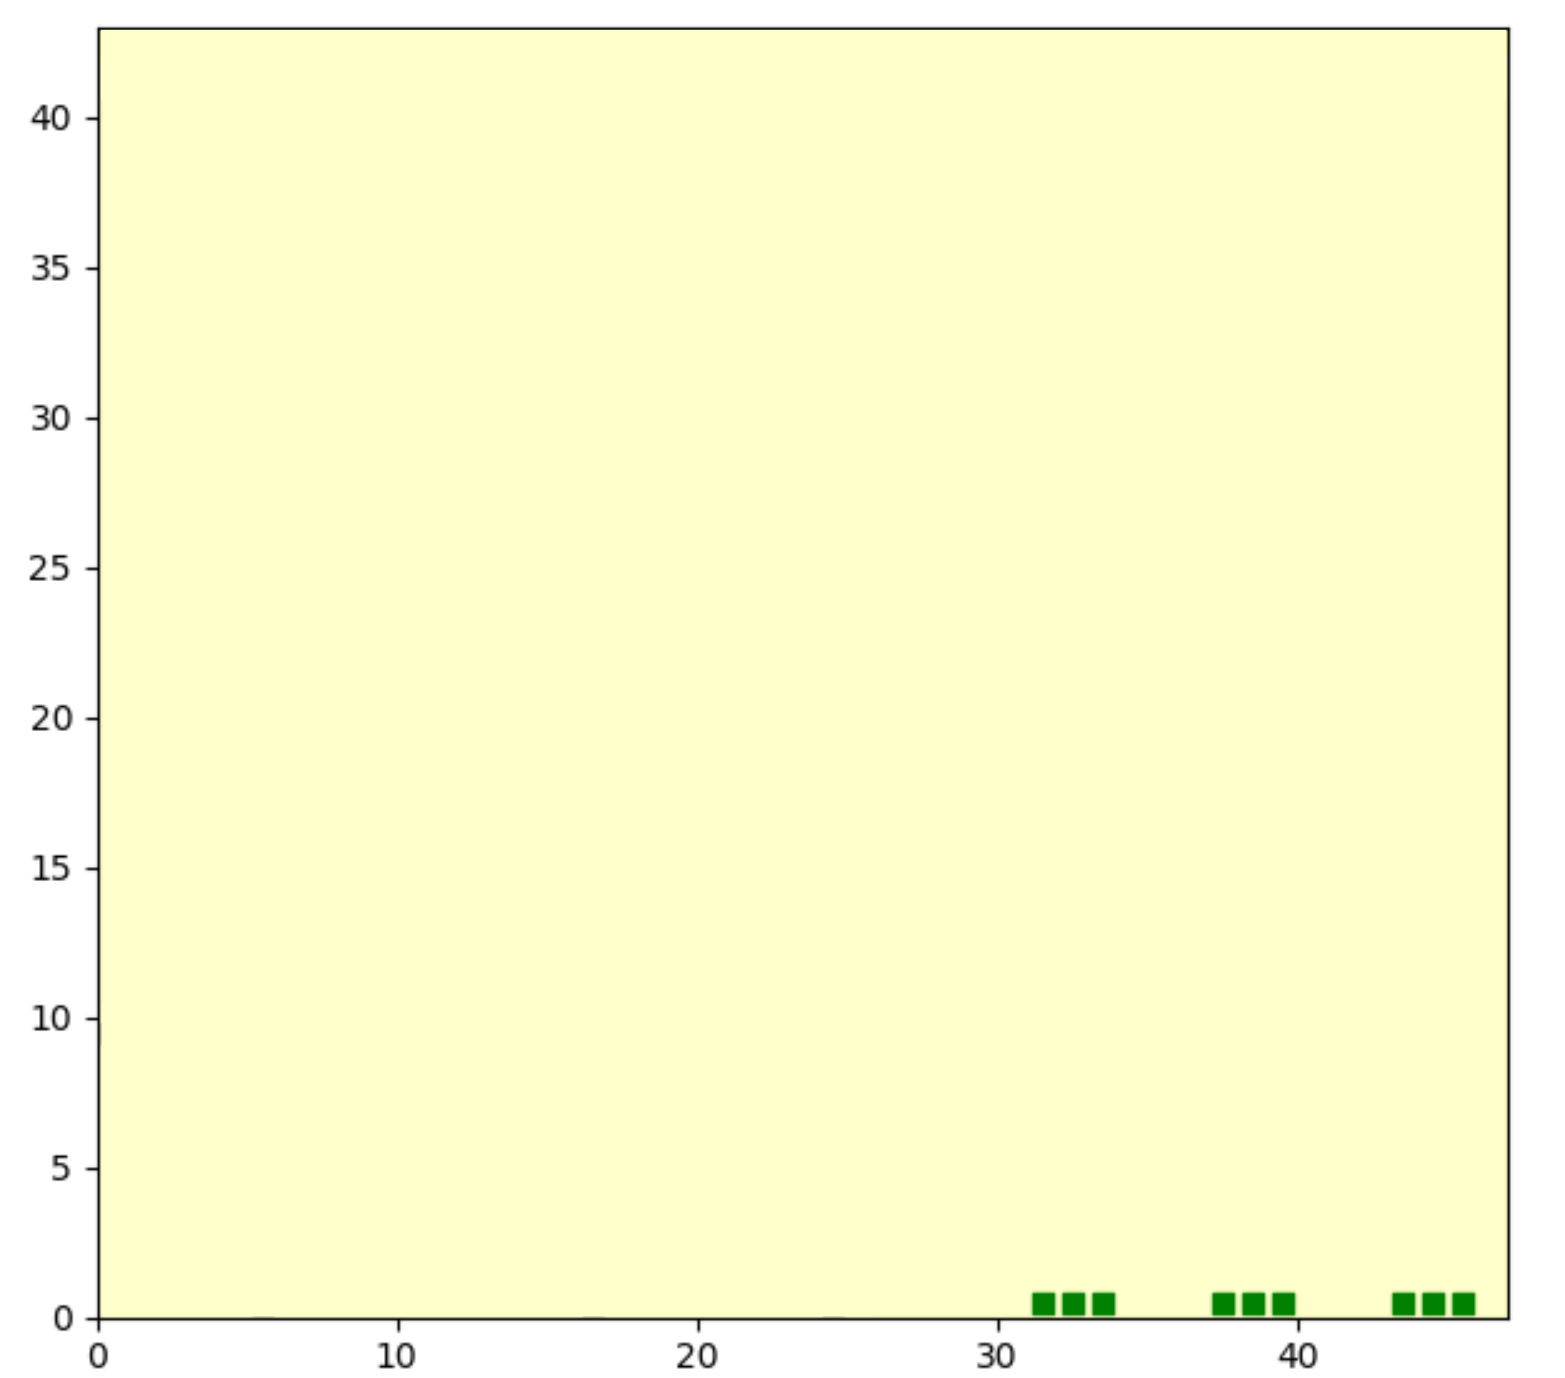
\includegraphics[width=\textwidth]{Figures/Map/Gates.png}
\end{minipage}
\hspace{0.5cm}
\begin{minipage}[ht]{0.45\linewidth}
\centering
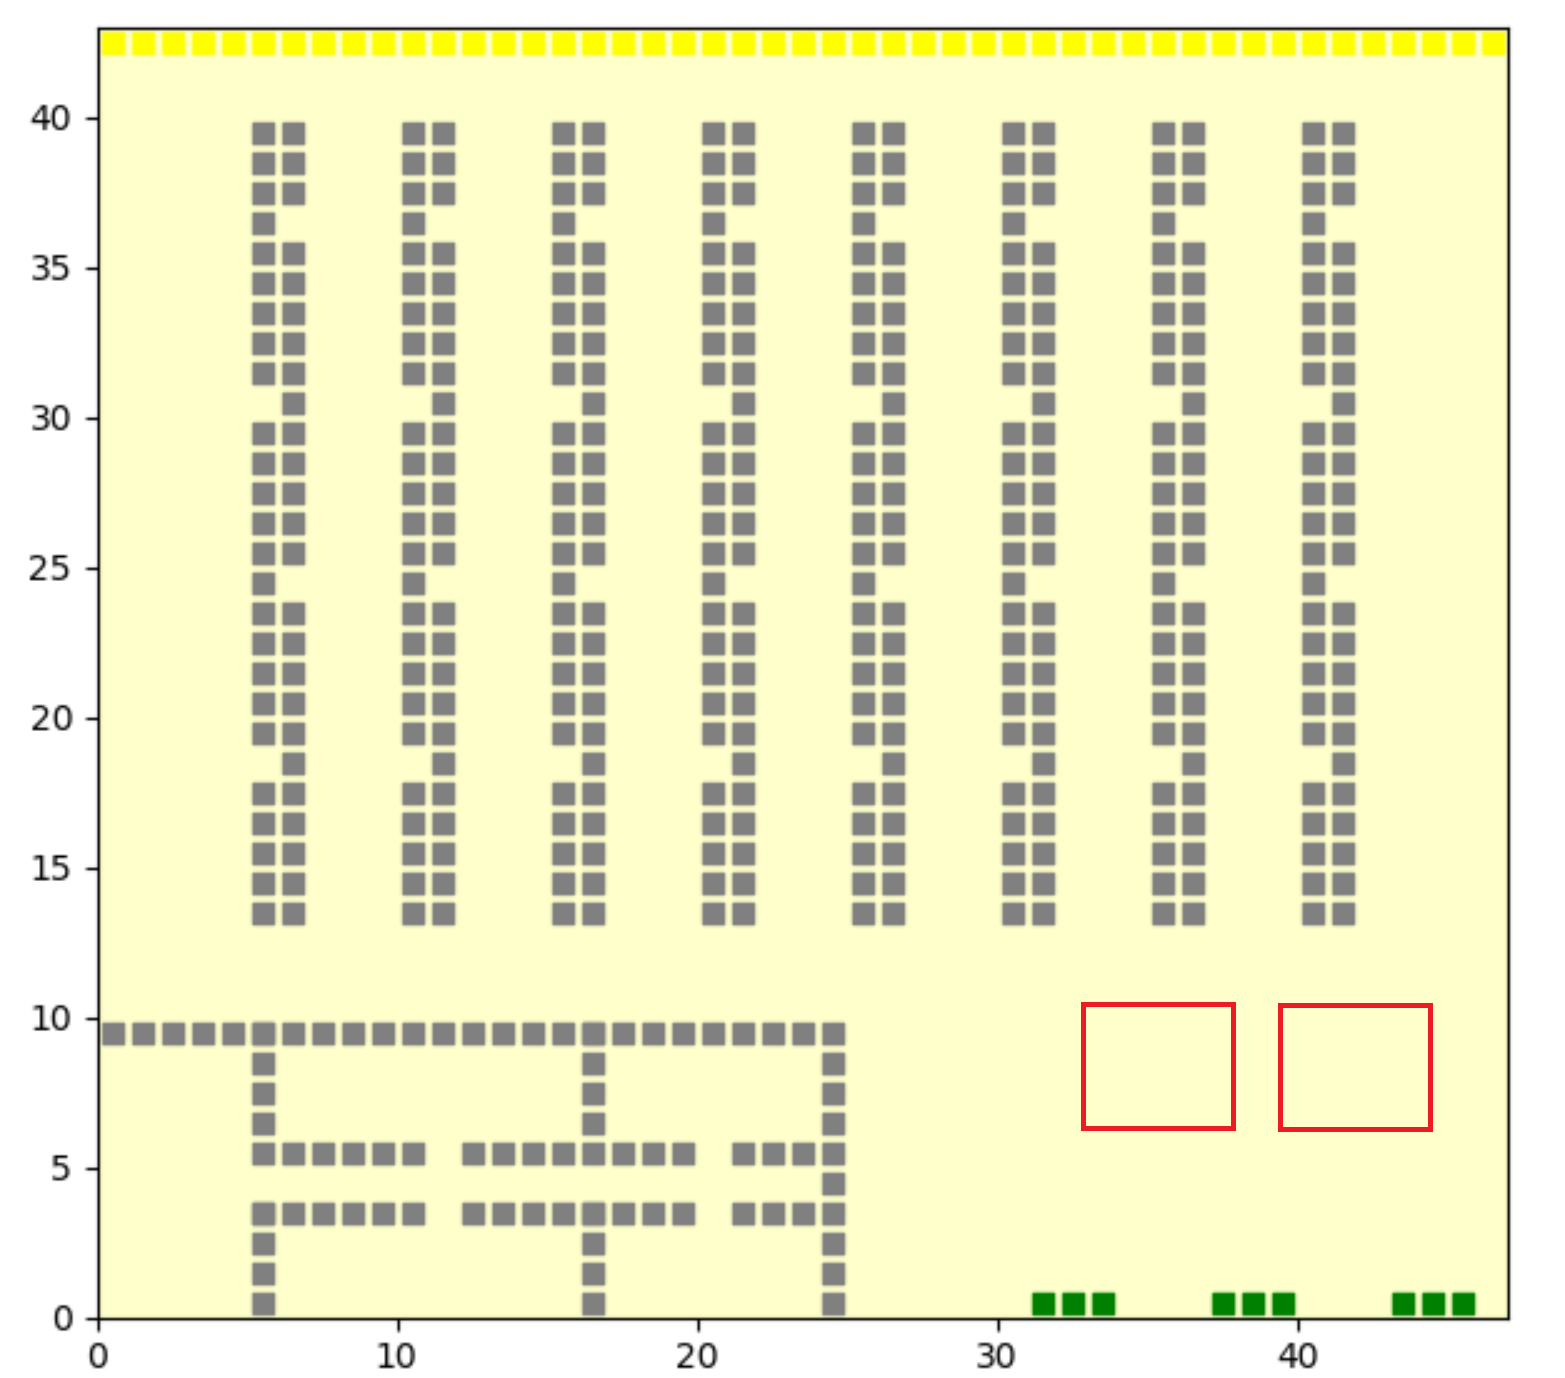
\includegraphics[width=\textwidth]{Figures/Map/WaitingArea.png}
\end{minipage}

\begin{minipage}[ht]{0.45\linewidth}
\vspace{0.2cm}
\textbf{Punti di scarico:} Rappresentati con il colore verde. Questi sono i punti in cui verranno rilasciate le merci prelevate dagli AGV in precedenza.
\end{minipage}
\hspace{0.5cm}
\begin{minipage}[]{0.45\linewidth}
\vspace{0.2cm}
\textbf{Area di attesa:} Indicata con due rettangoli rossi di fronte ai punti di scarico. Gli AGV in attesa di scaricare attenderanno qui il loro turno.
\end{minipage}

\begin{minipage}[ht]{0.45\linewidth}
\centering
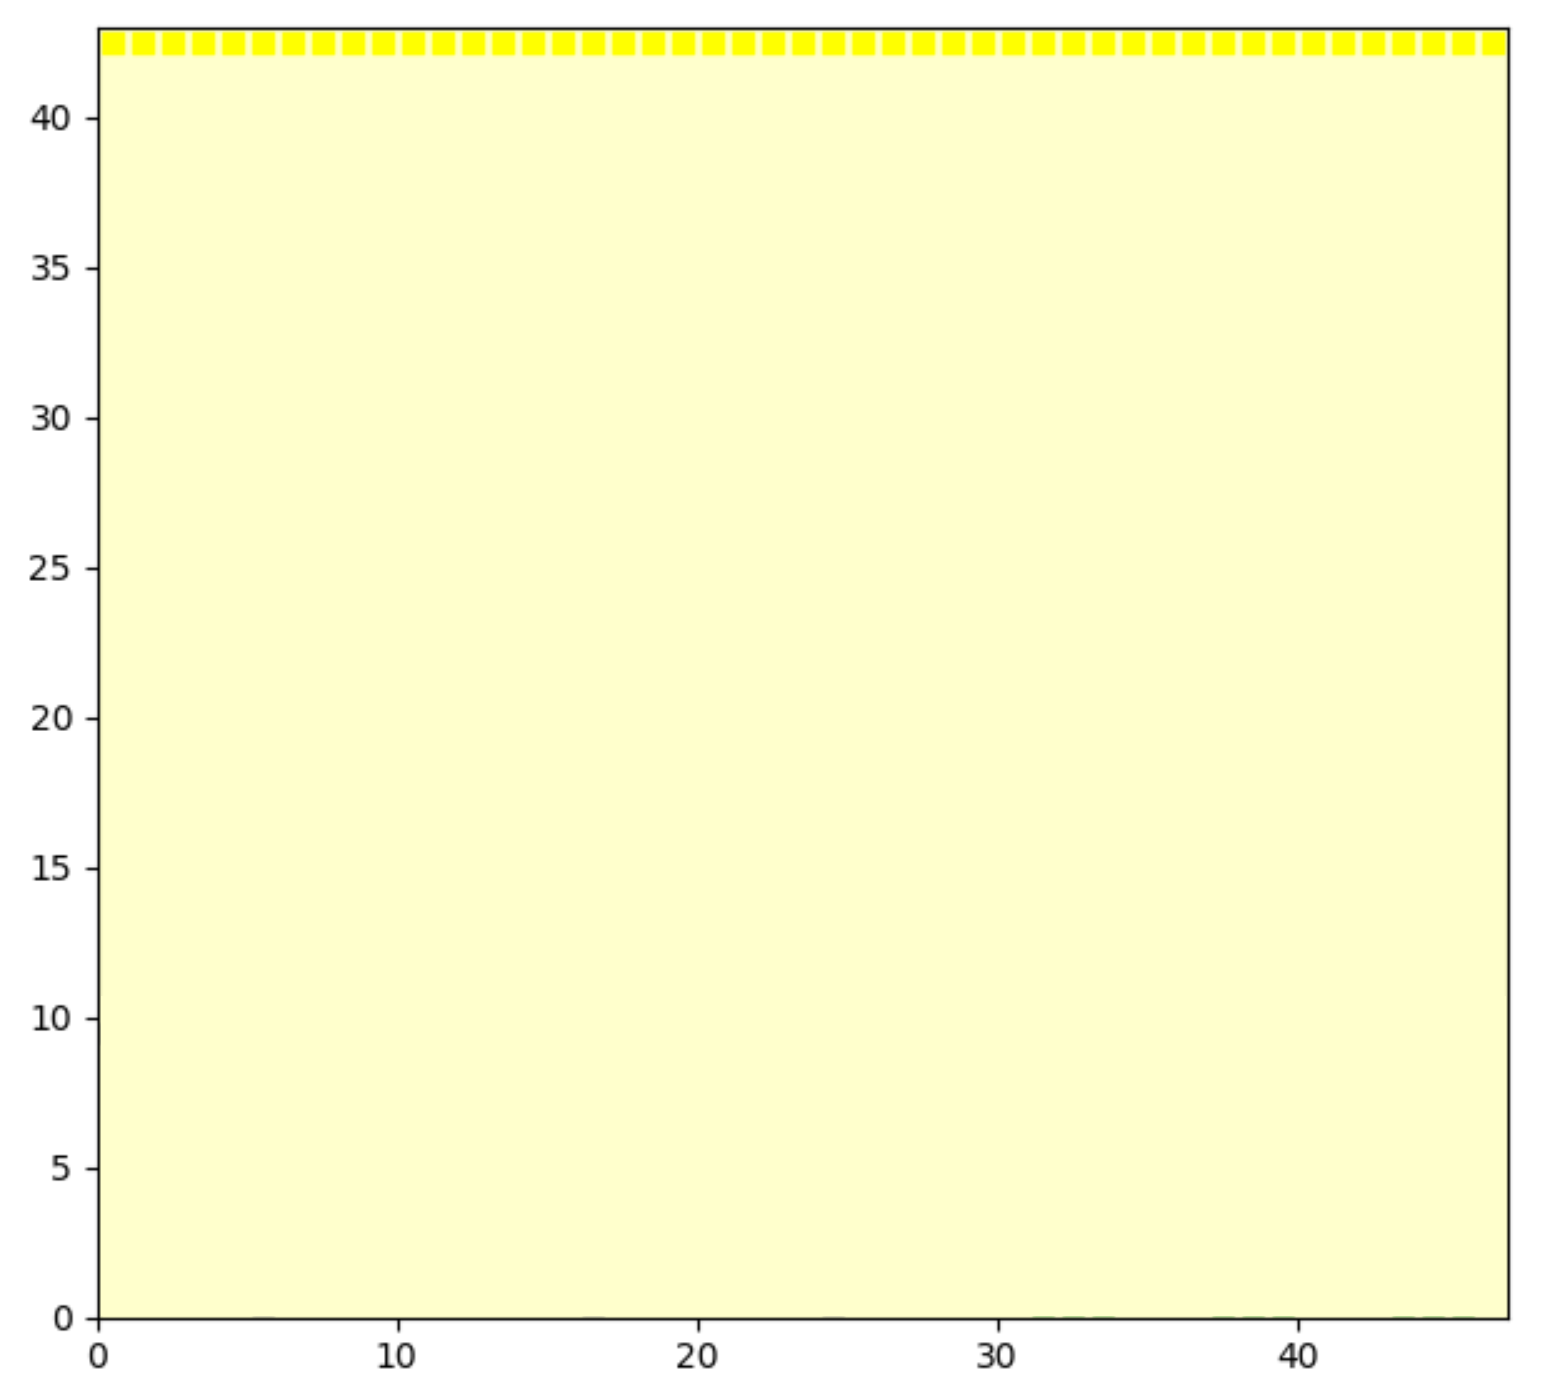
\includegraphics[width=\textwidth]{Figures/Map/ChargingStation.png}
\end{minipage}
\hspace{0.5cm}
\begin{minipage}[ht]{0.45\linewidth}
\centering
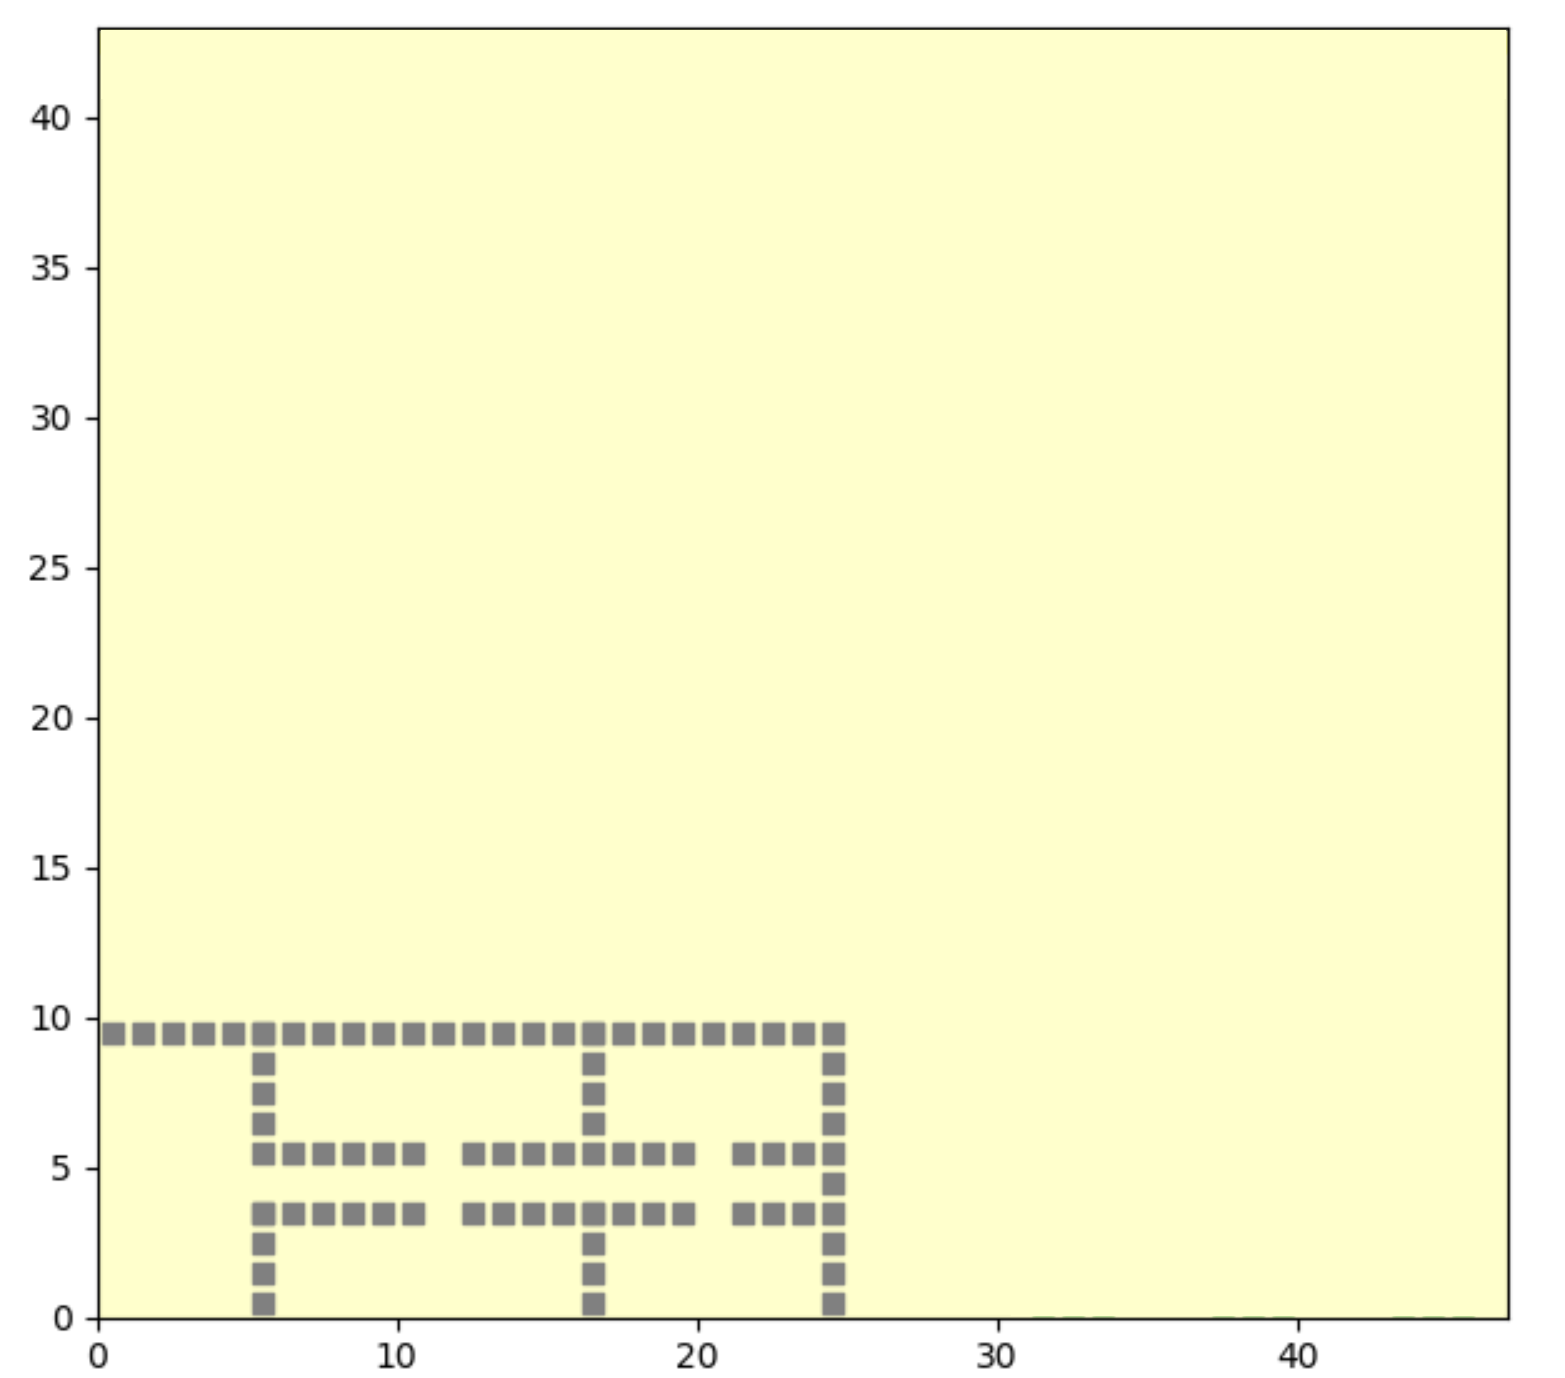
\includegraphics[width=\textwidth]{Figures/Map/Offices.png}
\end{minipage}

\begin{minipage}[ht]{0.45\linewidth}
\vspace{0.2cm}
\textbf{Area di ricarica:} Rappresentate con il colore giallo in alto all'interno dell'ambiente di simulazione. Durante questo lavoro sono state utilizzate solamente come punto di partenza degli AGV per la simulazione e per possibili lavori futuri.
\end{minipage}
\hspace{0.5cm}
\begin{minipage}[ht]{0.45\linewidth}
\vspace{0.2cm}
\textbf{Uffici:} Rappresentati con il colore grigio in basso a sinistra all'interno dell'ambiente di simulazione. Non hanno uno scopo effettivo bensì sono stati riportati per rimanere coerenti con la mappa originale del magazzino e non considerare spazi effettivamente non disponibili.
\end{minipage}

\newpage

\subsection{Modellazione AGV}
Ciascun AGV presente all'interno della simulazione è caratterizzato da:
\begin{itemize}
\item Id:
\item Colore:
\item Posizione:
\item Posizione iniziale:
\item Stato:
\item Info sull'ordine:
\item Cliente:
\item Percorso:
\item Gate:
\item Goal:
\item Articoli prioritari:

\end{itemize}
\subsubsection{Algoritmo di navigazione}
Navigazione libera. Algoritmo A*.

\subsubsection{Gestione dei conflitti}

\newpage

\subsubsection{Stati assumibili}
\begin{itemize}
    \item \textbf{Free}: Stato iniziale di ogni AGV. In questo stato l’AGV prende a carico, in base al tipo di comportamento scelto per la simulazione, il primo oggetto da prendere.
    \item \textbf{ToGoal}: l’AGV ha preso in carico un oggetto da prendere e si muove verso il punto di prelievo per quel pacco. Una volta arrivato a destinazione, inizierà a caricare quest’ultimo.
    \item \textbf{Loading}: l’AGV è fermo in un punto di prelievo e carica un pacco. In base alla disponibilità di un punto di scarico per quel pacco, decide se andare al punto di scarico, o al WP del Gate nel quale dovrebbe scaricare.
    \item \textbf{ToGate}: l’AGV si appresta a portare il pacco verso il punto di scarico di un Gate per scaricarlo.
    \item \textbf{ToWaitP}: l’AGV si muove verso un WP. Ogni turno, però, controlla se un punto di scarico di un Gate è ora libero e, in quel caso, cambia direzione andando verso il Gate libero. Questo, però, se e solo se non sono presenti altri AGV in coda  per quel punto di scarico lui (AGV in stato “Wait”)
    \item \textbf{Wait}: l’AGV è fermo in un WP e aspetta che si liberi un Gate per consegnare un pacco. Ogni turno controlla se un Gate è libero e, se è così, inizia a muoversi verso il punto di scarico del Gate
    \item \textbf{Unloading}:  l’AGV è fermo in un punto di scarico e scarica un pacco in un Gate. Se sono presenti altri oggetti che necessitano di essere portati ad un gate, di competenza dell’AGV, viene assegnato il nuovo pacco all’AGV che, altrimenti, mette come prossimo obiettivo il ritorno alla postazione di ricarica.
    \item \textbf{ToHome}: l’AGV ha completato gli ordini di sua competenza e si appresta a tornare alla posizione di ricarica da cui è partito (Home)
    \item \textbf{Home}: l’AGV è fermo in posizione iniziale
\end{itemize}

\newpage

\subsubsection{Transizioni tra stati}
La seguente immagine permette di farsi una chiara idea degli stati che può assumere un AGV (già riportati poco sopra nella sezione AGV) e come può passare da uno stato all'altro in base al verificarsi di determinati eventi.
\begin{figure}[ht]
\centering
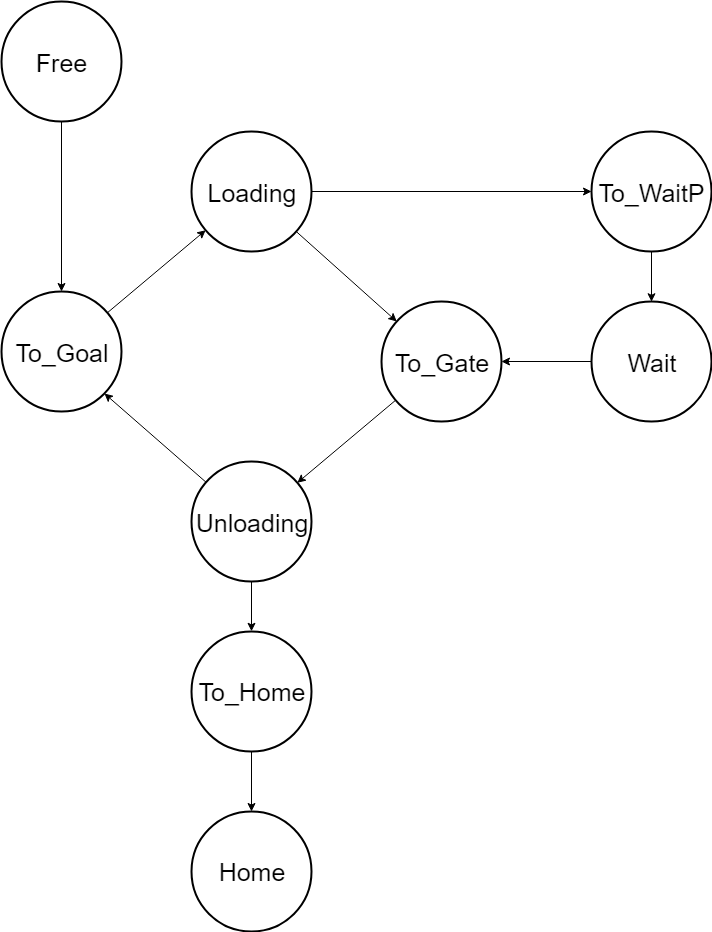
\includegraphics[width=0.75\textwidth,keepaspectratio]{Figures/Graphics/State_Transaction.png}
\caption[Transazioni tra stati di un AGV]{Transazioni tra stati di un AGV}
\label{fig:agv_states}
\end{figure}

\newpage

\subsection{Metodo di gestione ordini}
\subsubsection{Behaviour type 1}
Ciascun AGV esegue un singolo ordine.
\subsubsection{Behaviour type 2}
Ciascun AGV si occupa solamente di un certo gruppo di articoli.
\subsubsection{Behaviour type 3}
Ciascun AGV si occupa del primo articolo necessario al completamente degli ordini all'interno della lista in maniera progressiva.

\newpage
%%%%%%%%%%%%%%%%%%%%%%%%%%%%%%%%%%%%%%%%%%%%%%%
% AImplementazione
%%%%%%%%%%%%%%%%%%%%%%%%%%%%%%%%%%%%%%%%%%%%%%%
\section{Implementazione simulatore} 


\newpage
%%%%%%%%%%%%%%%%%%%%%%%%%%%%%%%%%%%%%%%%%%%%%%%
% Simulazione 
%%%%%%%%%%%%%%%%%%%%%%%%%%%%%%%%%%%%%%%%%%%%%%%
\section{Simulazione} % Main chapter title

Questa fase si pone l'obiettivo di simulare il funzionamento dei vari comportamenti implementati nelle fasi precedenti andando a prendere un set di ordini in input predefinito e un numero di AGV variabile, raccogliendo dati statistici riguardanti le simulazioni per permettere un analisi complessiva delle performance.

\subsection{Configurazioni simulate}
In particolare, si è deciso di eseguire la simulazione su 12 diverse configurazione in modo da poter andare ad analizzare i risultati al variare del comportamento e del numero di AGV.
Le configurazioni eseguite sono state quindi 12 e sono riportate di seguito:
\begin{itemize}
\setlength\itemsep{0.1em}
    \item \textbf{} Behaviour type 1 - Number of AGV 3 / 6 / 9 / 12
    \item \textbf{} Behaviour type 2 - Number of AGV 3 / 6 / 9 / 12
    \item \textbf{} Behaviour type 3 - Number of AGV 3 / 6 / 9 / 12
\end{itemize}

\subsection{Lista degli ordini per simulazione}
La lista di ordini considerata per effettuare la simulazione del sistema è stata scelta in maniera semi arbitraria. Come prima cosa infatti è stato indispensabile aggregare articoli appartenente a classi diverse nella stessa classe oppure al contrario dividere una singola classe di articoli in più sottoclassi. Tutto ciò ha permesso di ottenere un numero di classi adeguato alla simulazione sul sistema implementato. \newline
Successivamente si sono selezionati N ordini casuali da quelli disponibili, mantenendo invariate le distribuzioni di classi degli articoli all'interno di essi.\\

\noindent E' possibile notare come gli ordini che indirizzati al cliente "CO" sono di gran lunga più numerosi rispetto a quelli indirizzati a "FI" e "MI": questo rispecchia la distribuzione di ordini suddivisi per cliente presente all'interno degli ordini realmente raccolti dalla logistica.

\begin{figure}[ht]
\centering
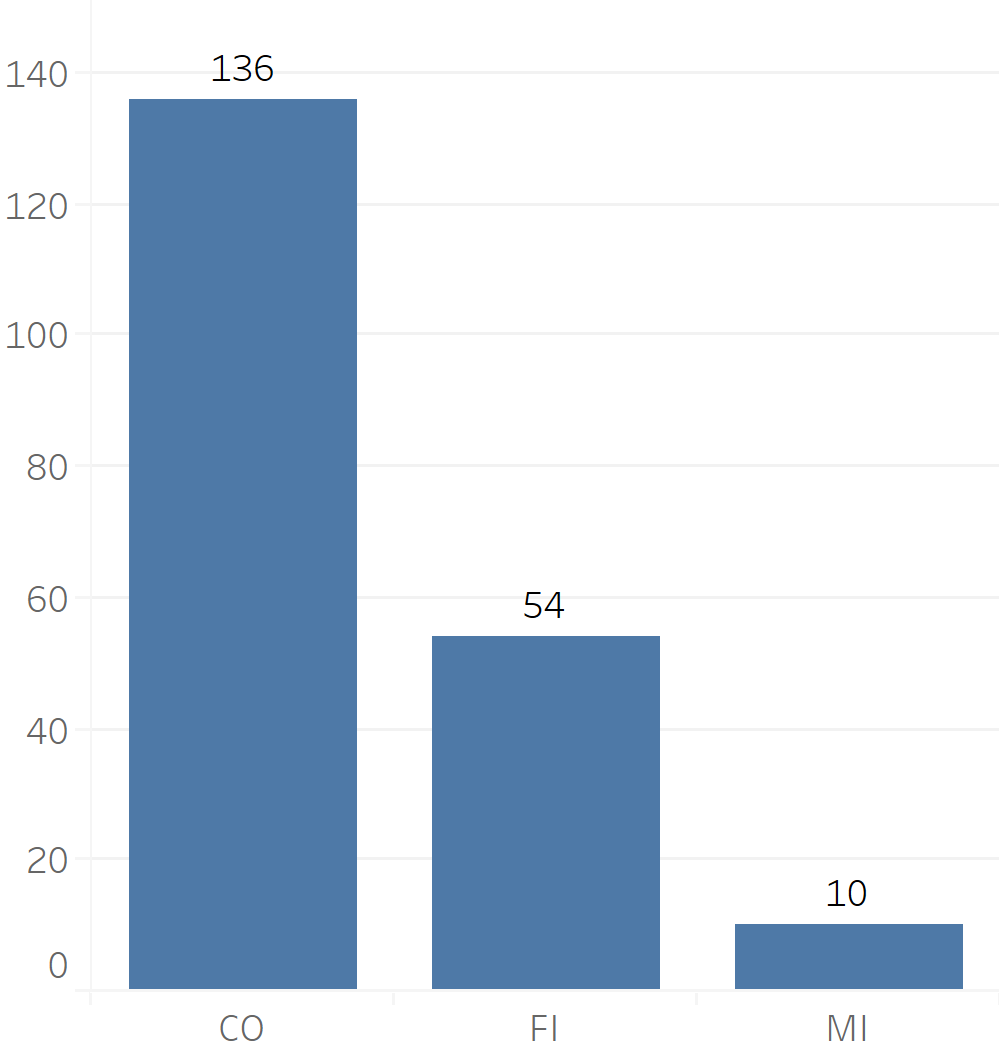
\includegraphics[width=0.6\textwidth,keepaspectratio]{Figures/Graphics/Orders_simulation.png}
\captionof{figure}[Numero di ordini associati ad ogni cliente]{Numero di ordini associati ad ogni cliente.}
\label{fig:OrdiniSimulazione}
\end{figure}

\noindent Inoltre è possibile vedere dai seguenti grafici come alcuni articoli compaiono molto più spesso all'interno di determinati clienti rispetto ad altri. 
\noindent Tutto ciò è stato mantenuto di proposito all'interno della lista degli ordini utilizzata per la simulazione in modo tale da renderla il più verosimile possibile e andare a considerare tutte quelle esigenze realmente presenti all'interno del contesto analizzato.

\begin{figure}[ht]
\centering
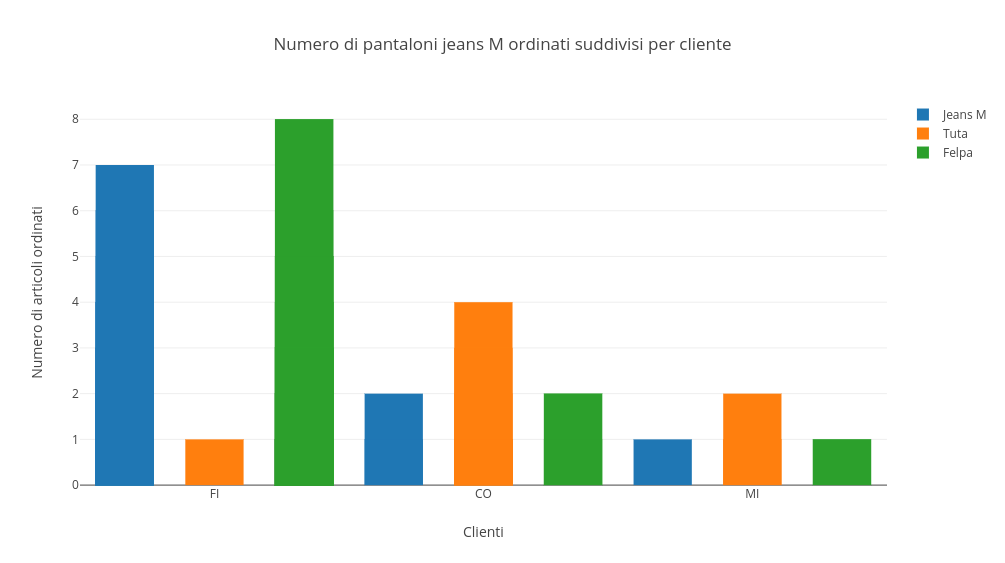
\includegraphics[width=0.8\textwidth,keepaspectratio]{Figures/Graphics/articoli_clienti.png}
\caption[Numero di diversi articoli per cliente]{Numero di diversi articoli ordinati per cliente}
\label{fig:Electron}
\end{figure}



\newpage

\subsection{Parametri di valutazione}
Per poter valutare le performance di ciascuna configurazione è stato implementato un sistema di raccolta delle statistiche significative. In particolare, questo sistema permette di raccogliere i dati relativi a:

\begin{itemize}
    \item \textbf{Conflicts:} numero di conflitti che sono stati rilevati durante la configurazione per ogni singolo AGV.
    \item \textbf{Conflict Wait:} numero di conflitti che sono stati rilevati durante la configurazione per ogni singolo AGV e che sono stati risolti con un AGV in attesa per un turno.
    \item \textbf{Conflict Path:} numero di conflitti che sono stati rilevati durante la configurazione per ogni singolo AGV e che sono stati risolti con un AGV che ricalcola il percorso per la sua destinazione.
    \item \textbf{Waiting Gate:} numero di timestep trascorsi da ciascun AGV all'interno delle aree di attesa.
    \item \textbf{Articles:}  numero di articoli elaborati, e quindi portati ad uno specifico gate, da ciascun AGV.
    \item \textbf{Moving Steps:} numero di step, ovvero di spostamenti da una cella ad un'altra adiacente, di ciascun AGV.
\end{itemize}

Questi parametri sono stati raccolti ad ogni timestep della simulazione per ogni singolo AGV per ogni configurazione, così da poter analizzare i risultati che si otterrano secondo diversi punti di vista.


\newpage
%%%%%%%%%%%%%%%%%%%%%%%%%%%%%%%%%%%%%%%%%%%%%%%
% Analisi dei risultati 
%%%%%%%%%%%%%%%%%%%%%%%%%%%%%%%%%%%%%%%%%%%%%%%
\section{Analisi dei risultati}

Questa fase si pone l'obiettivo di analizzare i dati raccolti dalla fase precedente di simulazione, con lo scopo finale di determinare quale risulta la configurazione migliore: prima di procedere è indispensabile però dare una definizione di "configurazione migliore". \newline
Sicuramente una configurazione può essere considerata più performante di un'altra se impiega meno tempo per portare a termine la stessa mole di lavoro. Andando però a consideraro solo il tempo impegato si trascurano alcuni aspetti che sono indispensabili per una azienda reale come in questo caso. E' infatti indispensabile trovare anche un giusto compromesso sul numero di AGV, dato che rappresentano un costo non indifferente di acquisto e gestione da parte delle aziende. \newline 
Questo numero di AGV ideale si può andare a determinare considerando alcuni dei parametri raccolti nella fase di simulazione: infatti, nel caso in cui ci fosse un valore molto alto per quanto riguarda il parametro Waiting Gate significherebbe che alcuni AGV resi operativi sono rimasti in zona di attesa a lungo, e tutto ciò significa uno spreco di risorse. \newline
\newline
Lo scopo di questa fase quindi è proprio quello di individuare quali parametri permettono di dichiarare che una configurazione è migliore rispetto un'altra, tenendo ben presente il contesto lavorativo ed economico in cui questa ricerca è collocata. 

\subsection{Dati raccolti dalle simulazioni}
In questa sezione sono riportati, descritti e analizzati alcuni dei grafici generati dai dati raccolti durante la fase di simulazione e che sono stati considerati più rilevanti nel raggiungimento dello scopo di questa sezione. \newline

FASE MOLTO IMPORTANTE CHE VA AD ANALIZZARE LE COSE PIUì IMPORTANTI SUI DATI RACCOLTI. POI I GRAFICI E COME VISUALIZZARLI SI GENERANO.. FA NIENTE PER IL MOMENTO

\begin{itemize}
    \item \textbf{Conflicts: } osservazioni sui conflitti.. dove sono di più, perchè, infieriscono su performance? relativi grafici 
    \item \textbf{Waiting Gate: } osservazioni sulle attese.. dove sono di più, perchè, infieriscono su performance? relativi grafici 
    \item \textbf{Waiting Gate: } osservazioni sulle attese.. dove sono di più, perchè, infieriscono su performance? relativi grafici 
\end{itemize}

\begin{figure}[!htb]
\minipage{0.49\textwidth}
  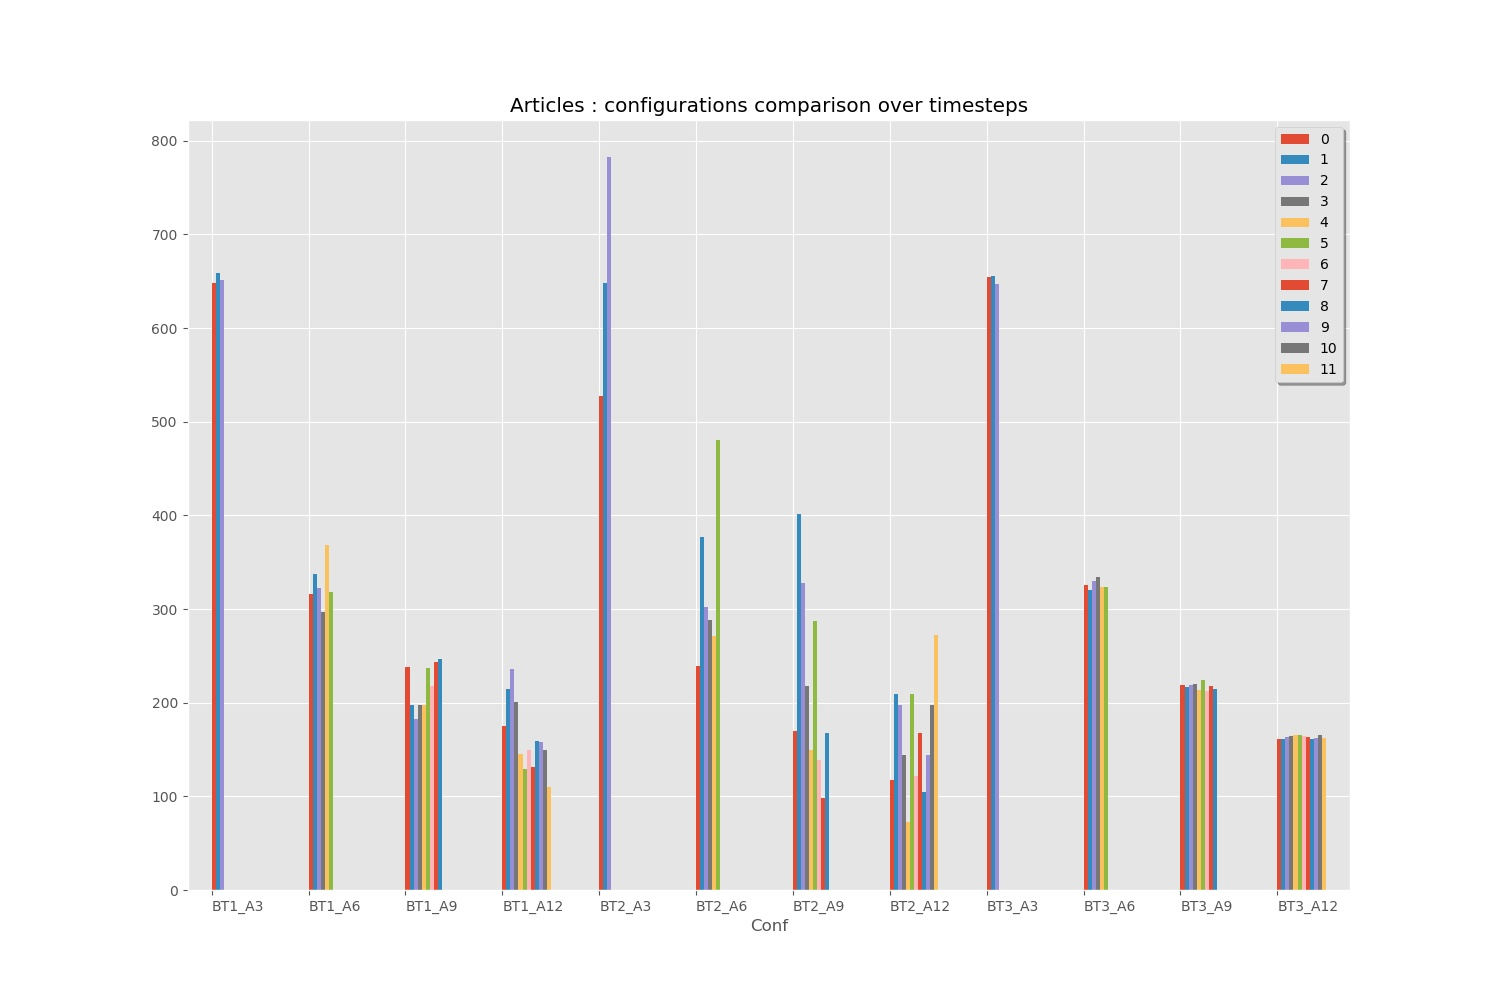
\includegraphics[width=\linewidth]{Figures/Results_Graphics/AGV_Articles.jpg}
  \caption{A really Awesome Image}\label{fig:awesome_image1}
\endminipage\hfill
\minipage{0.49\textwidth}
  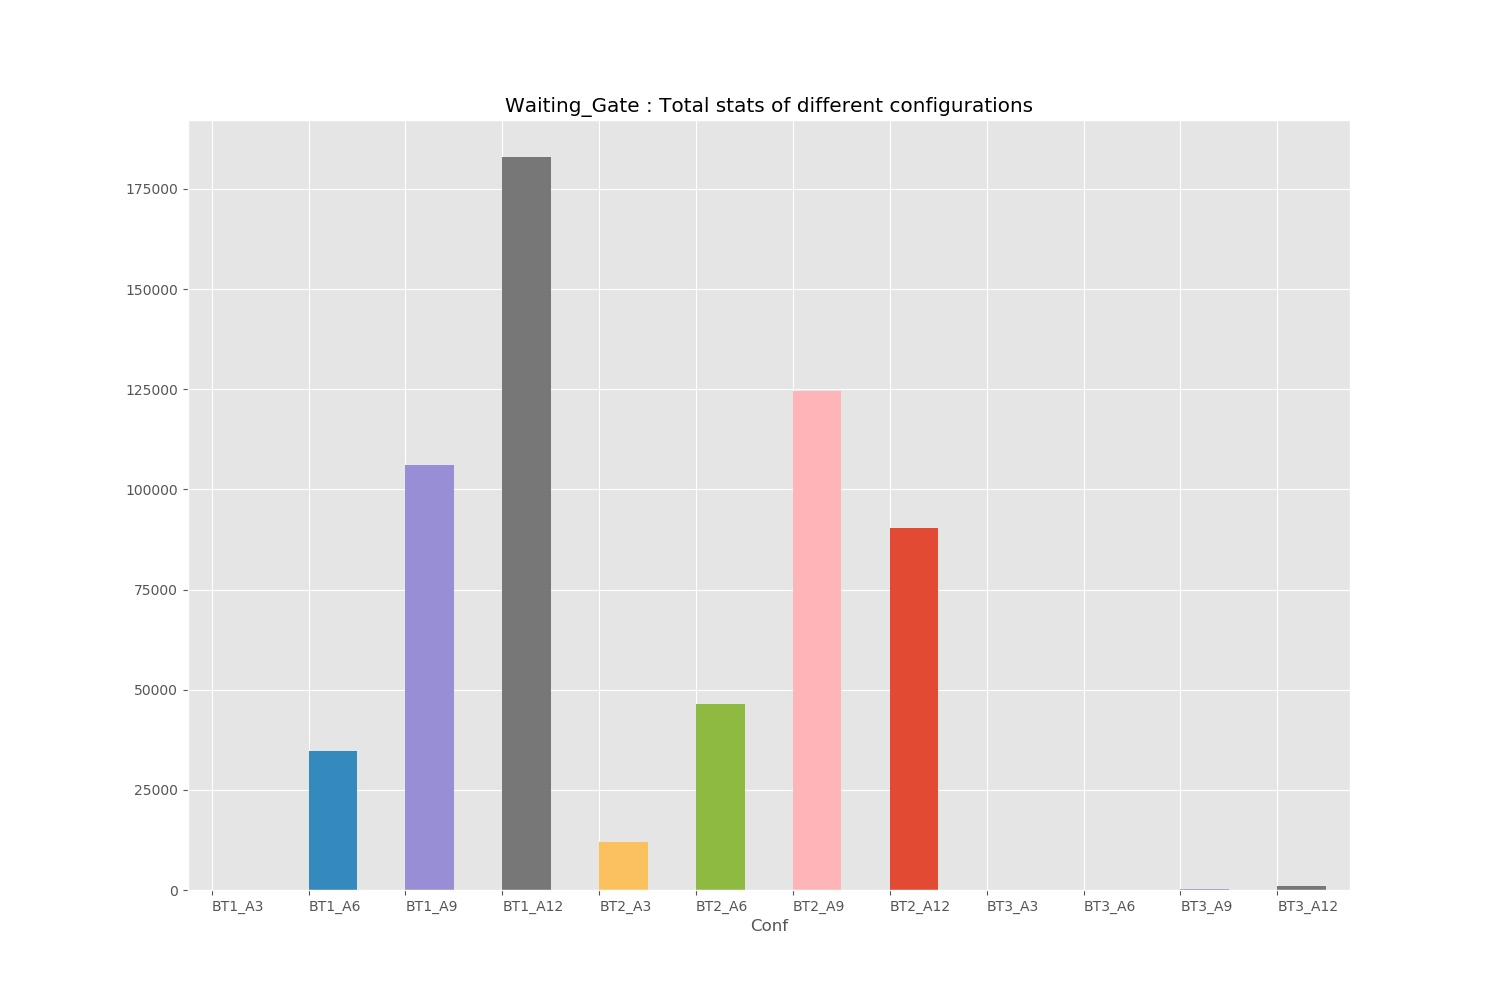
\includegraphics[width=\linewidth]{Figures/Results_Graphics/Total_Waiting_Gate.jpg}
  \caption{A really Awesome Image}\label{fig:awesome_image2}
\endminipage\hfill
\minipage{1\textwidth}%
  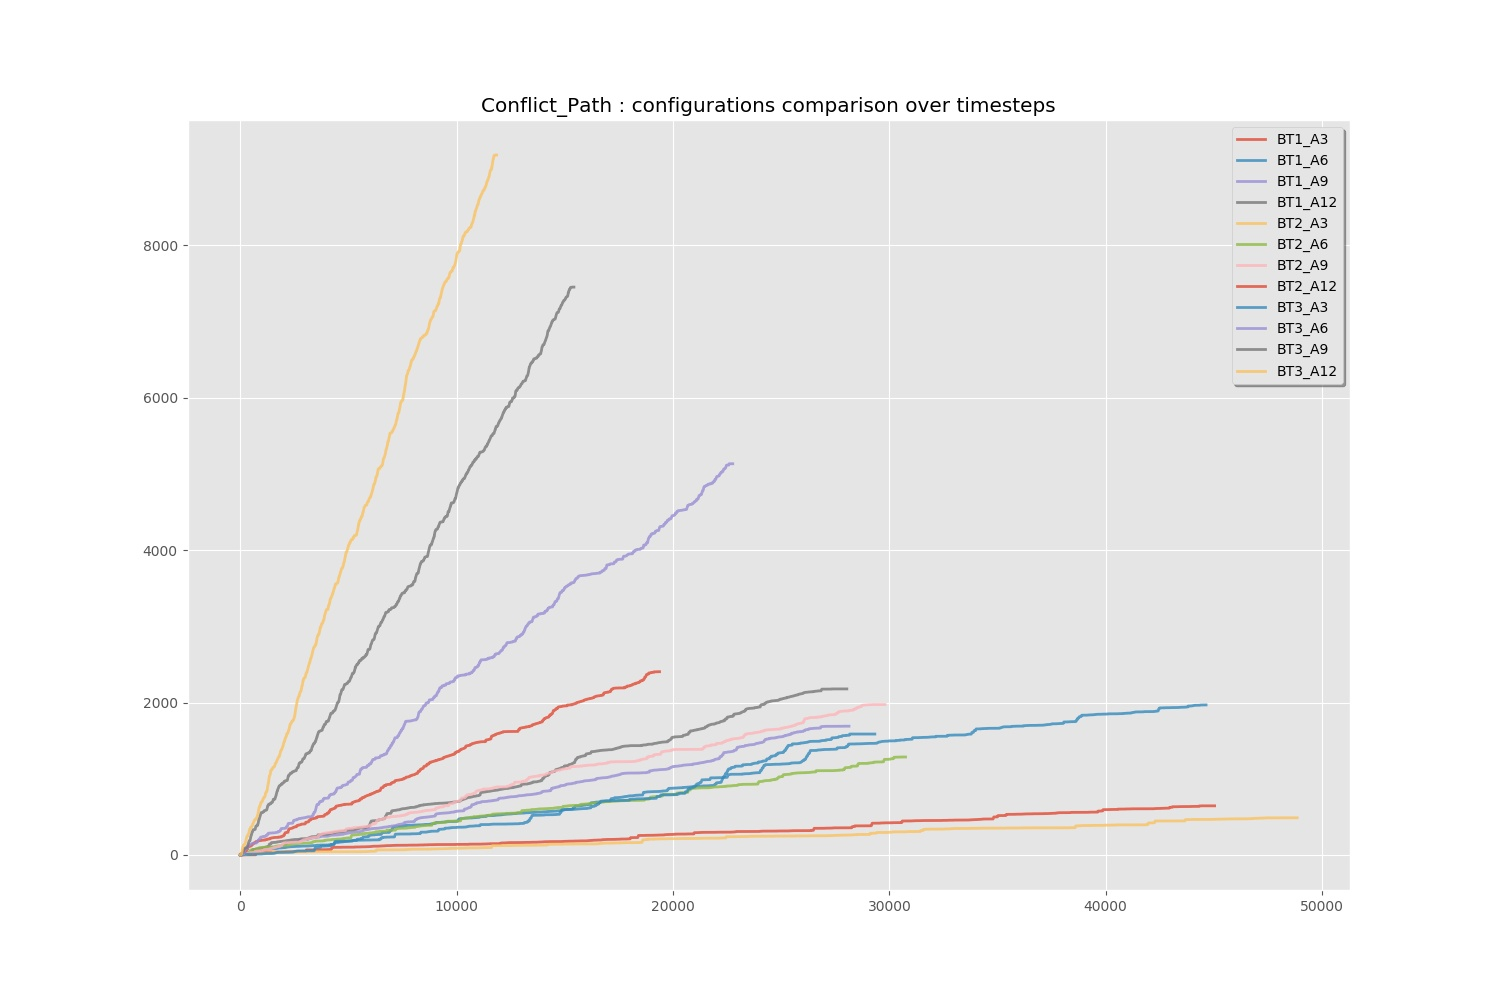
\includegraphics[width=\linewidth]{Figures/Results_Graphics/Timestep_Conflict_Path.jpg}
  \caption{A really Awesome Image}\label{fig:awesome_image3}
\endminipage
\end{figure}


\newpage
%%%%%%%%%%%%%%%%%%%%%%%%%%%%%%%%%%%%%%%%%%%%%%%
% CONCLUSIONI 
%%%%%%%%%%%%%%%%%%%%%%%%%%%%%%%%%%%%%%%%%%%%%%%
\section{Conclusioni}

\subsection{Lavori e sviluppi futuri}
Gestione della batteria \newline
Gestione di danni o rotture AGV

\newpage
%%%%%%%%%%%%%%%%%%%%%%%%%%%%%%%%%%%%%%%%%%%%%%%
% BIBLIOGRAFIA 
%%%%%%%%%%%%%%%%%%%%%%%%%%%%%%%%%%%%%%%%%%%%%%%\\
\bibliographystyle{amsplain}
\bibliography{references}

\end{document}